%%% Local Variables:
%%% mode: latex
%%% TeX-master: t
%%% End:

\documentclass[master, openany, oneside]{tongjithesis}
%开始用了openright,但这样即每章都是奇数页开始,但实际上,只需要摘要、目录、英文摘要、正文第一章、
%参考文献、附录、个人简历都从奇数页开始即可,正文内部章节可以从偶数页开始,因此用\cleardoublepage命令实现

% \documentclass[%
%   master|doctor, % mandatory option
%   xetex|pdftex|dvips|dvipdfm, % optional
%   secret,
%   openany|openright,
%   arialtoc,arialtitle]{tongjithesis}

% 所有其它可能用到的包都统一放到这里了,可以根据自己的实际添加或者删除。
\usepackage{tongjiutils}
\usepackage[top=1.3in,bottom=1.15in,left=1.25in,right=1.25in]{geometry}%调节每一页的页面大小,
\usepackage[figuresright]{rotating}
\usepackage{graphicx}
\usepackage{titlesec}
\usepackage{algorithmicx}
\usepackage{algpseudocode}
\usepackage{etex}
\usepackage[perpage,symbol*,bottom]{footmisc} %使用了\raggedbottom后仍然保持脚注在页面底部,且脚注在每一页都从1开始,
%符合规范,脚注形式为①,另外,此命令与下面命令还可以使得模板原先的自动填充的空白得到很好的控制,如果没有这个命令,
%章节标题与正文间的空白很难控制,特别是有图、表与公式的时候
\raggedbottom
\usepackage{epstopdf}
\usepackage{fancyhdr}
\usepackage{verbatim}
\usepackage{CJKpunct}
\usepackage{setspace}
\usepackage{longtable}
\usepackage{url}
\usepackage{pifont}
\usepackage{algorithm}
\usepackage{ulem}
\usepackage{extarrows}
\usepackage{caption}
\setlength\parskip{0pt}
\frenchspacing
\widowpenalty=10000
%此命令貌似是用来修改图标与正文的间距的


% 你可以在这里修改配置文件中的定义,导言区可以使用中文。
\def\myname{同济人}

\begin{document}

% 定义所有的eps文件在 figures 子目录下
\graphicspath{{figures/}}


%%% 封面部分
\frontmatter

%%% Local Variables:
%%% mode: latex
%%% TeX-master: t
%%% End:
%\secretlevel{保密} \secretyear{2}

\ctitle{你的标题}

% 按照申请工学学位设计。如有其它需要,请修改相应文字。
\makeatletter
  \iftongji@doctor
    \cdegree{工学博士}
  \else
    \iftongji@master
      \cdegree{工学硕士}
    \fi
  \fi

\makeatother

\cdepartment{电子与信息工程学院}

\snumber{10XXXXXXXXX}

\cmajorfirst{计算机科学与技术}

\cmajorsecond{计算机应用技术}

\cauthor{你的姓名}

\csupervisor{你的 教授}

% 如果没有副指导老师或者联合指导老师,把各自{}中内容留空即可。

\cassosupervisor{}

\ccosupervisor{}

% 日期自动生成,如果你要自己写就改这个cdate
%\cdate{\CJKdigits{\the\year}年\CJKnumber{\the\month}月}
\makeatletter
  \iftongji@doctor
    \edegree{Doctor of Philosophy}
  \else
    \iftongji@master
      \edegree{Master of Science}
    \fi
  \fi

\makeatother

\cfunds{(国家自然科学基金 (No.XXXXXXXX) 支持)}

\efunds{(Supported by the Natural Science Foundation of China for\\ Grant No.XXXXXXXXX)}

\etitle{Your title}

\edepartment{School of Electrical and Informational Engineering}

\emajorfirst{Computer Science and Technology}

\emajorsecond{Computer Application Technology}

\eauthor{Tongji Ren}

\esupervisor{Prof. XXXXXX}

\eassosupervisor{}

% 这个日期也会自动生成,你要改么?
% \edate{May, 2009}

% 定义中英文摘要和关键字
\begin{cabstract}
树木建模一直是计算机图形学中一个极具挑战并且非常重要的研究课题。随着目前WebVR、WebGame、WebGIS等基于Web的应用
发展迅速,为了适应网络的传输以及用户日益增长的对图形效果的追求,如何使树木建模轻量化而富有真实感就变得尤为重要。
传统的3DSMAX、Maya等建模工具不仅耗费人力物力,而且输出的面片模型也体积庞大,不适合应用到Web领域。而诸如L-System
等基于规则的树木建模又由于其规则性而使树木模型缺失了真实感,这又不能满足用户对效果的需求。怎样在真实感和轻量化之间
进行权衡的问题亟待解决。

为了解决这个矛盾,本课题提出了一套高效、低成本,的分级轻量化树木建模方法。这里的分级轻量化体现为其对应用的适应性。
即可以基于不同应用对轻量化的不同要求,在尽可能保证真实感的前提下进行轻量化,以产生最终符合要求的模型尺寸。这种可分级
的轻量化树木建模方法还可以进一步被扩展为自动适应网络带宽条件或用户硬件条件而自动产生最匹配的轻量化树木模型的方法。

为了实现高效的分级轻量化建模方法,本文首先将PyrLK光流法进行基于仿射变换和反向追踪的改进,并且将其运用到三维重建
的特征点匹配步骤中,以提高树木特征点的匹配率和稳定性。然后进行GPU加速的三维重建以得到高精度点云模型。接着本文
运用三维体素泛洪和最小二乘线性拟合的方法对树木骨架和半径信息进行抽取,以适应树木生长规律的方法抽取出了准确的骨架。
然后本文提出了根据应用对轻量化的需求等级,对骨架进行纵向和横向的合并,以减小骨架的尺寸来实现轻量化,从而更好地适应
面向网络的应用的需求。最后本文还给出了一套完整的基于图像树木建模的质量评价,提出了还原度的概念来客观、量化地评价建模出
的模型的还原度以及在轻量化过程中质量的丢失。
\end{cabstract}

\ckeywords{基于图像建模, 树木建模, 轻量化建模, 三维重建, 骨架抽取}

\begin{eabstract}
Tree modeling has long been a challenging subject in computer graphics. As the Web-oriented applications(WebVR, WebGame,
WebGIS, etc) develop rapidly and the persuit of graphics effect increases quickly, the lightweight and realism of tree modeling are badly
needed nowadays. The traditional 3d modeling tools such as 3DSMAX and Maya are not only time and labour consuming, but it
takes a large model size, which are not practical to Web apps. The rule-based modeling such as L-System can solve the size
problem, but its output lacks realism, which is not tolerated by users. So the balance between realism and lightweight
is a real problem which are eagerly demanded to solve.

In order to solve this problem, a high-efficiency, low-cost and lightweight-classified tree modeling method is proposed.
Here the lightweight-classified means it can produce different lightweight levels of tree models. And to implement this 
goal, this method will reduce model size on the premise of not losing much realism. This method can also be applied furthur
to automatically adapt to the bandwidth and hardware conditions of the client side.

For implementing the lightweight method, we first improve the traditional PyrLK optical flow method to support affine transformation
and backward feature tracking, which can furthur be applied to do feature matching in gpu accelerated 3D reconstruction and 
improve the match ratio. Then we use flooding algorithm in 3D voxel model and least squares method to discover the tree skeleton and
its radius information. According to the lightweight level the applications require, we reduce the model size by merging the
branches vertically and horizontally respectively. At last we propose a modeling quality evaluation method, which will objectively and 
quantizedly evaluate the restore degree of the tree model.
\end{eabstract}

\ekeywords{Image-based Modeling, Tree Modeling, Light-weight Modeling, PyrLK Optical Flow, Skeleton Extraction}

\makecover


% 目录

\tableofcontents

% 符号对照表
%\begin{denotation}
\item[GNU] GNU's Not Unix /'gnu:/
\item[GFDL] GNU Free Documentation License
\item[GPL] GNU General Public License
\item[FSF] Free Software Foundation
\item[SMP] 对称多处理
\item[API] 应用程序编程接口
\item[$E$] 能量
\item[$m$] 质量
\item[$c$] 光速
\item[$P$] 概率
\item[$T$] 时间
\item[$v$] 速度
\end{denotation}


%%% 以下索引按需要选择
% 插图索引
%\listoffigures
% 表格索引
%\listoftables
% 公式索引
%\listofequations

%%% 正文
\mainmatter

%%% Local Variables:
%%% mode: latex
%%% TeX-master: t
%%% End:



\chapter{引言}
\label{cha:intro}
\section{背景介绍}
\label{sec:background}
在互联网飞速发展的今天,网络应用已经延伸到生活的方方面面。微博、人人网、
在线购物、在线音乐等已经成为当今人们生活的一部分。面向Web的虚拟现实应用
如WebVR、WebGame、WebGIS等也必然将成为虚拟现实发展的重要方向。树木作为自然
界常见的事物,在各种虚拟现实的场景中出现的频率很高。然而树木形态各异,结构
复杂,给3D建模带来了很大的难度。通常单棵树的数据量已经不小,对于构建一个
树木的聚集场景(如森林)就更加庞大,这容易使得场景负荷变大而产生延迟。因此,
树木建模的质量和效率将直接决定面向Web的虚拟现实应用的成败。

目前的树木的3D建模,主要是通过专业的3D建模工具(3DSMAX、Maya等)进行手工建模。
这种建模方法对建模人员的要求较高,并且需要的时间长。而且这种方法通常最终生成
的是面片信息,要表达一棵形态复杂的树木需要大量的顶点信息,导致最终生成的模型
体积较大,对于需要大批树木的场景,负荷就会变得更大。

目前树木的轻量化建模,从最简单的基于分形,广告牌技术的建模到稍微复杂的基于
规则的建模,都存在一个共同的问题,就是在轻量化的同时,很大程度上舍弃了模型
的真实感和树木本身的形态特征。随着当今应用对真实度要求的升高,这类轻量化的
建模方法已经不能完全满足需求。真实感与轻量化之间的权衡也成为了当今应用需要
考虑的一个重要因素。

本课题基于以上的考虑,从基于图片对树木结构进行完整的恢复,到面向应用需要对
真实感与轻量化进行人工控制,到最后模型重建质量的评估,给出了一套完整的解决
方案。

\section{课题的主要工作}
\label{sec:objective}
本课题的主要工作有:

1. 对PyrLK光流法进行改良,并将其运用于三维重建算法中的特征点匹配步骤,使树木
重建的模型更加准确和精细。

2. 提出了基于三维体素泛洪和空间反向投影的三维重建方法,以连续的体素替代传统
方法不连续的点云,使得后续的骨架抽取步骤更加准确和方便。

3. 提出了基于多方向迭代和步长探索的树木骨架抽取方法。该方法区别于传统的3D瘦化
骨架抽取方法,它只适用于具有分形结构的3D骨架,所以更能够得到准确的树木骨架。

4. 提出了基于用户交互对树木模型进行完善和轻量化,让最终的应用来决定其所需的树木
模型,避免了主观的一味轻量化或一味追求真实感而带来的需求矛盾,将模型的成型延迟
至具体的应用。

5. 提出了基于图像的树木重建质量评估方法,对于建模质量和轻量化过程中真实感的下降
程度给出了函数化和量化的评价依据。


%%% Local Variables:
%%% mode: latex
%%% TeX-master: t
%%% End:



\chapter{中华人民共和国}
\label{cha:china}

\section{其它例子}
\label{sec:other}

在第~\ref{cha:intro} 章中我们学习了贝叶斯公式~(\ref{equ:chap1:bayes}),这里我们复
习一下:
\begin{equation}
\label{equ:chap2:bayes}
p(y|\mathbf{x}) = \frac{p(\mathbf{x},y)}{p(\mathbf{x})}=
\frac{p(\mathbf{x}|y)p(y)}{p(\mathbf{x})}
\end{equation}

\subsection{绘图}
\label{sec:draw}

本模板不再预先装载任何绘图包(如 \textsf{pstricks,pgf} 等),完全由你自己来决定。
个人觉得 \textsf{pgf} 不错,不依赖于 Postscript。此外还有很多针对 \LaTeX{} 的
 GUI 作图工具,如 XFig(jFig), WinFig, Tpx, Ipe, Dia, Inkscape, LaTeXPiX,
jPicEdt, jaxdraw 等等。

\subsection{插图}
\label{sec:graphs}

强烈推荐《\LaTeXe 插图指南》!关于子图形的使用细节请参看 \textsf{subfig} 的说明文档。

\subsubsection{一个图形}
\label{sec:onefig}
一般图形都是处在浮动环境中。之所以称为浮动是指最终排版效果图形的位置不一定与源文
件中的位置对应\footnote{This is not a bug, but a feature of
\LaTeX!},这也是刚使 用 \LaTeX{}
同学可能遇到的问题。如果要强制固定浮动图形的位置,请使用
\textsf{float} 宏包, 它提供了 \texttt{[H]}
参数,比如图~\ref{fig:heythere}。
\begin{figure}[H] % use float package if you want it here
  \centering
  
\includegraphics[height=2cm]{hello.jpg}
  \caption{插个图插个图}
  \label{fig:heythere}
\end{figure}

大学之道,在明明德,在亲民,在止于至善。知止而后有定;定而后能静;静而后能安;安
而后能虑;虑而后能得。物有本末,事有终始。知所先后,则近道矣。古之欲明明德于天
下者,先治其国;欲治其国者,先齐其家;欲齐其家者,先修其身;欲修其身者,先正其心;
欲正其心者,先诚其意;欲诚其意者,先致其知;致知在格物。物格而后知至;知至而后
意诚;意诚而后心正;心正而后身 修;身修而后家齐;家齐而后国治;国治而后天下
平。自天子以至于庶人,壹是皆以修身为本。其本乱而未治者 否矣。其所厚者薄,而其所
薄者厚,未之有也!

\hfill \pozhehao《大学》


\subsubsection{多个图形}
\label{sec:multifig}

如果多个图形相互独立,并不共用一个图形计数器,那么用 \verb|minipage| 或者
\verb|parbox| 就可以。否则,请参看图~\ref{fig:big1},它包含两个小图,分别是图~\ref{fig:subfig1}
和图~\ref{fig:subfig2}。推荐使用 \verb|\subfloat|,不要再用
\verb|\subfigure| 和 \verb|\subtable|。
\begin{figure} %[h]
  \centering%
  \subfloat[第一个小图形]{%
    \label{fig:subfig1}
    
\includegraphics[height=2cm]{tongji-fig-logo.png}}\hspace{4em}%
  \subfloat[第二个小图形。如果标题很长的话,它会自动换行,这个 caption 就是这样的例子]{%
    \label{fig:subfig2}
    
\includegraphics[height=2cm]{tongji-text-logo.png}}
  \caption{包含子图形的大图形}
  \label{fig:big1}
\end{figure}

古之学者必有师。师者,所以传道受业解惑也。人非生而知之者,孰能无惑?惑而不从师,
其为惑也,终不解矣。生乎吾前,其闻道也固先乎吾,吾从而师之;生乎吾後,其闻道也亦
先乎吾,吾从而师之。吾师道也,夫庸知其年之先後生於吾乎!是故无贵无贱无长无少,道
之所存,师之所存也。

嗟乎!师道之不传也久矣,欲人之无惑也难矣。古之圣人,其出人也远矣,犹且从师而问焉;
今之众人,其下圣人也亦远矣,而耻学於师。是故圣益圣,愚益愚。圣人之所以为圣,愚
人之所以为愚,其皆出於此乎?爱其子,择师而教之,於其身也,则耻师焉,惑焉。彼童子
之师,授之书而习其句读者,非吾所谓传其道、解其惑者也。句读之不知,惑之不解,或师
焉,或不焉,小学而大遗,吾未见其明也。巫医、乐师、百工之人不耻相师,  士大夫之族
曰“师”曰“弟子”之云者,则群聚而笑之。问之,则曰:彼与彼年相若也,道相似也,位
卑则足羞,官盛则近谀。呜呼!师道之不复,可知矣。巫医、乐师、百工之人。吾子不齿,
今其智乃反不能及,其可怪也欤!圣人无常师。孔子师郯子、苌子、师襄、老聃。郯子之徒,
其贤不及孔子。孔子曰:“三人行,必有我师。”是故弟子不必不如师,师不必贤於弟子。
闻道有先後,术业有专攻,如是而已。

如果要把编号的两个图形并排,那么小页就非常有用了:
\begin{figure}
\begin{minipage}{0.48\textwidth}
  \centering
  
\includegraphics[height=2cm]{tongji-whole-logo.png}
  \caption{并排第一个图}
  \label{fig:parallel1}
\end{minipage}\hfill
\begin{minipage}{0.48\textwidth}
  \centering
  
\includegraphics[height=2cm]{tongji-whole-logo.png}
  \caption{并排第二个图}
  \label{fig:parallel2}
\end{minipage}
\end{figure}

李氏子蟠,年十七,好古文、六艺,经传皆通习之,不拘於时,学於余。余嘉其能行古
道,作师说以贻之。

\hfill \pozhehao 韩愈(唐)


\chapter{基于图像的树木轻量化3D建模方法}
\label{cha:techroute}

\section{技术路线}
\label{sec:techroute}
本文提出了一套完整的基于图像的树木轻量化3D建模的方法。该方法首先以树木图片
序列作为输入,用经过改进的方法对树木进行三维重建,使三维重建得到的模型精确
度和完整性都得以提高。然后再用基于空间方向迭代和步长探索的方法抽取树木的骨
架,最终再基于用户交互对骨架进行改善与轻量化。

该技术路线旨在实现一个对建模设备和条件要求不高,适用于一般应用的方法。在方便
和简单的基础上,尽可能多的加入自动化,并结合少量用户交互,以实现高效、精确的
树木轻量化3D建模。

该方法的主要步骤如下:

\subsection{基于改进的PyrLK光流法的图像特征匹配}
\label{subsec:match}
本文首先将著名的金字塔LK光流法(PyrLK)进行了改进和扩展,使本来以平面平移作为
运动假设的PyrLK光流法扩展为以平面仿射变换为运动假设,这样便能在两帧以空间角度
旋转而拍摄的图片中,捕捉到空间旋转变换的投影,提高了匹配的完整性和正确性。之后
本文再将得到的匹配点进行反向匹配,只有在一定容错区间内的匹配点对才会被接纳,并且
进行中值阈值,将邻域相似度小于中值以及反向匹配度小于中值的匹配对剔除,以提高匹配
算法的鲁棒性。

\subsection{三维重建}
\label{subsec:calibration}
特征匹配完成以后,本文使用了美国华盛顿大学西雅图分校Changchang Wu的可视化运动
恢复工具VisualSFM来完成基于多张图片的树木三维重建。VisualSFM实现了SiftGPU(GPU加速)
和多核的捆集调整(Multicore Bundle Adjustment), 使得相机参数的恢复更加
快速和精确。在这个步骤本文用经过改进的PyrLK光流法的匹配结果替换VisualSFM中的
SIFT特征点匹配文件,进一步地改进了相机参数恢复的准确度和可信度。

%\subsection{基于体素泛洪与空间反向投影的三维重建}
%\label{subsec:3drec}

\subsection{基于三维体素泛洪与线性拟合的三维树木骨架抽取}
\label{subsec:treesklextract}
在完成了三维重建之后,将会得到一个比较完整的树木空间点云模型。本文根据该点云的
空间分布,并结合树木自底向上的自然生长规律和分形的逻辑结构特征,在阈值范围内,
进行三维的体素泛洪,同时向多个子方向进行迭代,不断增加步长来扩大邻域范围。在确定
邻域以后将几个点数比例较大的方向作为分支方向,并用线性拟合的方法确定其精确的分支
方向。在确定分支方向后,再根据点到线的距离和投影分别估算出半径和长度。
同时在迭代过程中及时剔除已经形成枝干的点云,来加速泛洪算法的完成。最终获取到的骨架信息
是含有父子关系的节点信息,相比起3DSMAX等手工工具导出的面片模型,这种逻辑结构的
模型大大的减小了其尺寸,但是由于逻辑结构并没有多少丢失,所以极具真实感。并且这种
结构更便于后续的处理和进一步轻量化。

\subsection{基于用户交互的模型改善与轻量化}
\label{subsec:userinteraction}
由前面方法所得到的树木三维骨架虽然已经是含有父子信息的树木逻辑结构,但是由于前面
的步骤都是自动化生成,所得到的结果不可能100\%地保证符合具体应用的需求。并且前面的
骨架信息虽然比起用面片来表示树木模型已经大大的轻量化了,但是针对实际的应用,本文
还可以根据用户的交互来合并分支,从而进一步对模型进行轻量化,以适用于轻量化要求更
高的应用。

\subsection{建模质量评估}
\label{subsec:qualityevaluation}
对于一个通过建模获得的树木模型,如果没有一个客观的量化评价指标,就无法从客观的角度
反馈树木模型的还原度和各个步骤算法的可行性。本文提出了建模还原度的概念,以模型重建
的还原度来量化的表现建模的质量。该还原度分别计算输入图像序列的信息量、三维重建的还原
度和骨架抽取的还原度。并将它们有机地结合起来形成了最后总的建模还原度。

\section{技术路线图}
\label{sec:techrouteimg}
\begin{figure}[H]
	\centering
	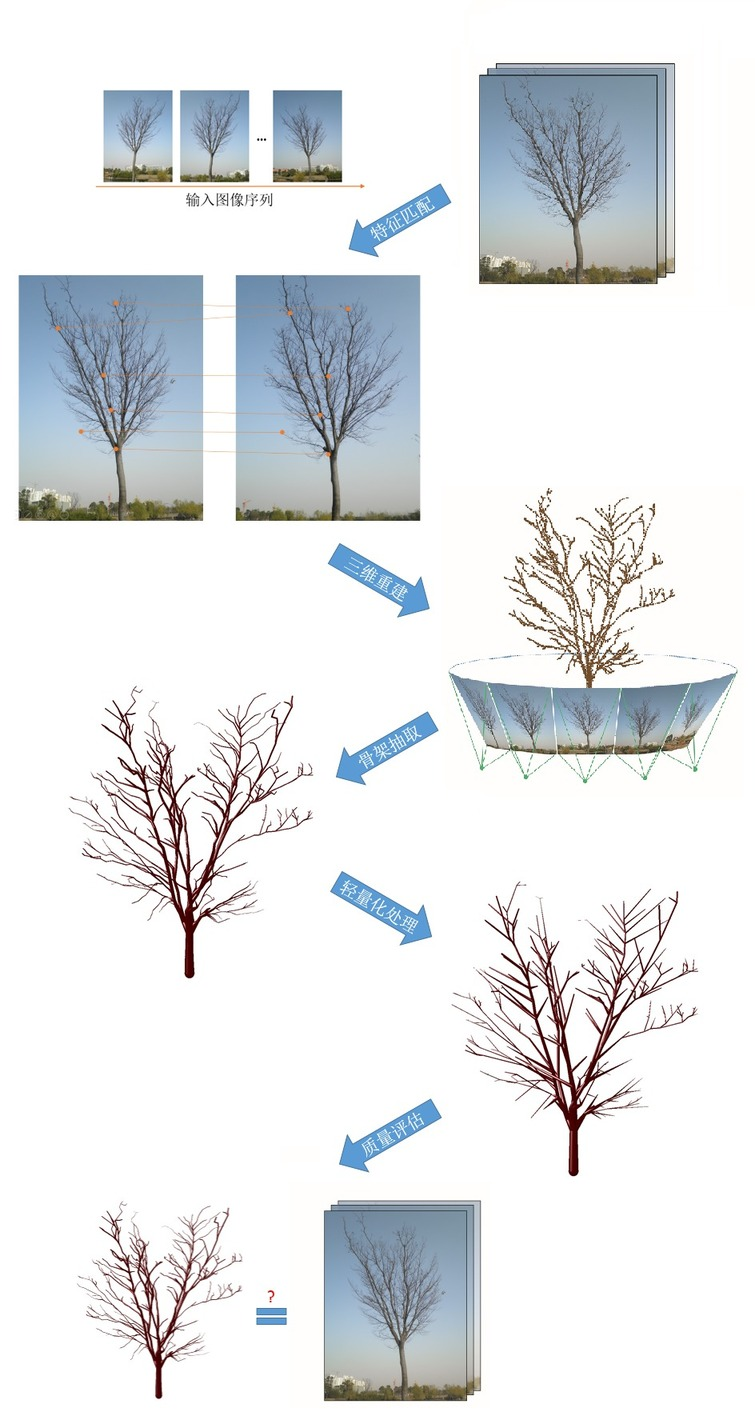
\includegraphics[height=18cm]{techroute.jpg}
	\caption{技术路线图}
	\label{fig:techroute}
\end{figure}


\chapter{基于图像树木轻量化建模的若干算法}
\label{cha:algorithm}
%----------------------------------PyrLK--------------------------------------
\section{基于改进的PyrLK光流法的特征点匹配方法}
\label{sec:pyrlk}
基于图像的树木建模第一步是三维重建,而三维重建的第一步则是特征点的匹配。
所谓的特征点匹配,是在多张图片中找到空间同一个点在其上的投影位置,从而为三维
重建的后续步骤提供数据支持。这里的特征点,本文选择了具有平移和旋转不变性的
Harris角点,以便用已有的方法快速找出图片中的特殊位置点。然后再结
合改进的PyrLK光流法,对找到的Harris角点进行3D匹配,这里的匹配不只是一般地
基于邻域平移假设的匹配,而是支持平面仿射变换假设的匹配,并且对在容错区间以外
的匹配结果进行了剔除,保证了匹配的精确性和可信度。最后本文将匹配的结果存储到
匹配文件以供后续使用。

%\subsection{对于SIFT特征点匹配的尝试}
%对于特征点的匹配,本文首先尝试的是利用VisualSFM工具自带的SIFT特征点匹配。
%但是经过大量实验发现,该工具自带的SIFT特征点匹配并不能很完整地找到匹配的
%点对,从而导致了三维重建所依赖的数据不足、不精确,最后重建出来一个缺失度
%很大的模型,这样的模型显然不能成功的进行骨架抽取。
%
%根据实验结果分析,除开

\subsection{光流法简介}
光流的概念最早是由James Gibson提出的。1981年,Horn和Schunck创造性地将二维速度
场和灰度联系起来,提出了一种有效的光流计算方法\cite{horn}。基于亮度不变的假设,
图像灰度分布的变化由背景或目标的运动引起,背景或目标的灰度不随时间变化。在这种
假设中,光流法通过目标和背景的不同速度来检测运动目标。

进一步说,将三维空间中的目标和场景对应于二维图像平面运动时,他们在二维图像平
面的投影就形成了运动,这种运动以图像平面亮度模式表现出来的流动就称为光流(Optical Flow)。
也就是说,光流是空间运动物体在观测成像面上对应像素点运动的瞬时速度,这个速度在
图像中以每秒像素点的位移个数来衡量,它巧妙地运用2D的灰度变化来表征3D物体的位置和
结构变化。而光流场(Optical Flow Field)就是所有光流点的集合,是一个2D瞬时速度场。
光流场能够表征整个图像的位移变化,从而对3D运动目标进行检测和跟踪。

在光流法提出以后,很多学者对其进行了研究和改进,并且它们的方法各具特点,算法性能
和运用场景各异。其中颇具代表性的是Lucas-Kanade局部平滑法(LK光流法)\cite{lk},它用基于
微分的方法,利用时变图像灰度的时空微分来计算速度矢量,并且加以图像平滑处理,来进行
光流跟踪。后来在2000年Jean-Yves又提出的基于图像金字塔实现的LK光流法,称为PyrLK光流法\cite{pyrlk}。

\subsection{PyrLK光流算法}
\label{subsec:pyrlk}
假设图片上的像素点的值函数为$I(x,y,t)$,表示坐标位于$(x,y)$的像素点在时刻$t$的像素值
为$I(x,y,t)$。那么经过$\Delta t$时间后,像素值将变为$I(x+\Delta x,y+\Delta y, t+\Delta t)$。
有如下推导:\\
\[  I(x+\Delta x,y+\Delta y, t+\Delta t)=I(x,y,t) + \frac{\partial I}{\partial x}\Delta x 
		+ \frac{\partial I}{\partial y}\Delta y + \frac{\partial I}{\partial t}\Delta t \]
\begin{displaymath}
	\begin{array}{cc}
		\implies & \frac{\partial I}{\partial x}\Delta x 
		+ \frac{\partial I}{\partial y}\Delta y + \frac{\partial I}{\partial t}\Delta t = 0\\
		\implies & \frac{\partial I}{\partial x}V_x 
		+ \frac{\partial I}{\partial y}V_y + \frac{\partial I}{\partial t} = 0 
	\end{array}
\end{displaymath}
\begin{equation}\label{eq:opticalflow}
	\begin{array}{cc}
				\implies & I_xV_x + I_yV_y = -I_t
	\end{array}
\end{equation}

Lucas-Kanade光流法算法基于以上原理,并假设两帧图像之间发生的位移是微量的,而且在一个
点的邻域内这个位移量是常数。这样可以对一个以$p$点为中心的窗口内的像素点写出一个光流方程
组,表征局部图像的运动向量$(V_x,V_y)$需要满足以下方程组:\\
\begin{equation}
	\left\{
		\begin{array}{c}
			I_x(q_1)V_x + I_y(q_1)V_y = -I_t(q_1)\\
			I_x(q_2)V_x + I_y(q_2)V_y = -I_t(q_2)\\
			\vdots\\
			I_x(q_n)V_x + I_y(q_n)V_y = -I_t(q_n)\\
		\end{array}
	\right.
\end{equation}

这里的$q_1,q_2,...,q_n$是局部窗口内的点,$I_x(q_i),I_y(q_i),I_z(q_i)$是图片$I$对$x,y,t$的
偏导函数在$q_i$处的值。将其写为矩阵形式得:\\
\begin{equation}
	A=	
	\left(
	\begin{array}{cc}
		I_x(q_1) & I_y(q_1)\\
		I_x(q_2) & I_y(q_2)\\
		  \vdots & \vdots\\
		I_x(q_n) & I_y(q_n)
		\end{array}
	\right),\quad
	v=
	\left(
	\begin{array}{c}
		V_x\\
		V_y
	\end{array}
	\right),\quad
	b=
	\left(
	\begin{array}{c}
		-I_t(q_1)\\
		-I_t(q_2)\\
		\vdots\\
		-I_t(q_n)
	\end{array}
	\right)
\end{equation}

这个方程组的方程个数远远多于未知数,所以$A$是过约束的,LK光流法运用最小二乘法来求解
出其光流速度。最小二乘法可以参考\ref{subsec:leastsquares}或查阅相关资料。

LK光流法虽然比较直观,但是存在一个问题,由于能够探测到的运动块的大小和所选窗口的大小呈正相关,为了
能够捕捉到大像素块的运动,需要将窗口大小相应调大。但是窗口大小越大,速度就需要在越大的邻域内保持稳定,
就越不符合光流在小范围内稳定的假设。基于金字塔的LK光流法是Lucas-Kanada方法的一种改进版实现,它解决了
窗口大小的与大块运动捕捉的矛盾。其具体思想如下:

设$I$和$J$是两张灰度图片,$I(x)$和$J(x)$分别表示图片$I$和$J$在位置$(x,y)$处的灰度值。现
考虑图片$I$上的一点$\mathbf{u}=(u_x, u_y)$,特征追踪的目标就是找到图片J上的一点$\mathbf{v}
=\mathbf{u}+\mathbf{d}=(u_x+d_x,u_y+d_y)$,使得$I(\mathbf{u})$和$J(\mathbf{v})$“相似”。其中
向量$\mathbf{d}=(d_x,d_y)$表示图片在点$\mathbf{x}$处的光流速度。下面来定义基于邻域的相似,
设$\omega_x$和$\omega_y$是两个整数,将使得下面式子最小化的向量$\mathbf{d}$定义为光流速度:\\
\begin{equation}\label{eq:similarity}
	\epsilon(\mathbf{d})=\epsilon(d_x,d_y)=\sum_{x=u_x-\omega_x}^{u_x+\omega_x}\sum_{y=u_y-\omega_y}
	^{u_y+\omega_y}(I(x,y) - J(x+d_x,y+d_y))^2.
\end{equation}
其中邻域窗口大小为$(2\omega_x+1)\times(2\omega_y+1)$。式子的含义为寻找向量$\mathbf{d}$使得
$\mathbf{u}$和$\mathbf{v}$在邻域窗口大小内的差异最小化。

然后该方法将图像金字塔化,即将原图像作为最高分辨率层,逐步降低图像的分辨率,并作为新的一层,加入到
LK光流法的迭代序列。通过这样多分辨率图层,使得邻域窗口的大小在低分辨率图像对应的区域可以映射到高
分辨率图像的更大的像素区域,从而支持了大块运动。

\subsection{改进的PyrLK光流算法}
\label{subsec:revisedpyrlk}
\subsubsection{加入放射变换}
对于PyrLK光流算法,已经能够很好的解决几乎任何像素块大小由平移主导的匹配。然而,这并不足以完美地
解决树木上点的匹配问题。因为相邻的两帧图像要求在空间形成一定的夹角进行拍摄,这样在两帧图像上,
也一定会产生由空间旋转投影过后带来的平面旋转。而这样的变换在PyrLK光流算法里是无法解决的,因为PyrLK
只是简单的将点的匹配依赖于点的平移。所以,有必要对PyrLK光流算法进行由平移变换到放射变换的扩展。

假设两个点的匹配满足仿射矩阵$A$,那么有:\\
\begin{equation}
	\left(
	\begin{array}{c}
		\Delta x'\\
		\Delta y'\\
		0
	\end{array}
	\right)
	=
	\left(
	\begin{array}{ccc}
		a_{11} & a_{12} & a_{13}\\
		a_{21} & a_{22} & a_{23}\\
				0 & 0 & 0
	\end{array}
	\right)
	\cdot
	\left(
	\begin{array}{c}
		\Delta x\\
		\Delta y\\
		1
	\end{array}
	\right)
\end{equation}
将其代入式\ref{eq:opticalflow}得:\\
\begin{equation}
	(a_{11}\ a_{12}\ a_{13}\ a_{21}\ a_{22}\ a_{23})\cdot
	\left(
	\begin{array}{c}
		\frac{\partial I}{\partial x}\Delta x\\
        \frac{\partial I}{\partial x}\Delta y\\
        \frac{\partial I}{\partial x}\\
        \frac{\partial I}{\partial y}\Delta x\\
        \frac{\partial I}{\partial y}\Delta y\\
        \frac{\partial I}{\partial y}\\
	\end{array}
	\right)
	=-I_t
\end{equation}

运用最小二乘法可以得到$A$的解。

将PyrLK中的定义式\ref{eq:similarity}稍作修改可可使得其支持仿射变换:\\
\[ Let\quad \mathbf{a_1}=(a_{11},a_{12},a_{13})\quad \mathbf{a_2}=(a_{21},a_{22},a_{23})\quad
\mathbf{b}=(d_x,d_y,1)\]\\
\begin{equation}\label{eq:affine}
	\epsilon(\mathbf{d})=\epsilon(d_x,d_y)=\sum_{x=u_x-\omega_x}^{u_x+\omega_x}\sum_{y=u_y-\omega_y}
	^{u_y+\omega_y}(I(x,y) - J(x+\mathbf{a_1}\cdot \mathbf{b},y+\mathbf{a_2}\cdot \mathbf{b}))^2.
\end{equation}


\subsubsection{提高鲁棒性}
本文前面几个小节一直在探讨如何改进和完善匹配的方法,从而提高精度和匹配可信度。然而,
这其中有一个问题,单方向的去追踪匹配点是否就能确定该两个匹配点真正的匹配呢?其实不然,
要确定两个点完全符合之前算法描述的特点,还需要反向进行检查,看$\mathbf{u}$和$\mathbf{v}$之间
的匹配是否是双向和可逆的。换句话说,本文之前定义的“相似”其实是单方面的$\mathbf{u}$相似于
$\mathbf{v}$,而$\mathbf{v}$是否相似于$\mathbf{u}$还不得而知。因此,考虑到算法的完整性和鲁棒性,
有必要进行反向的匹配来确定它们完全匹配。或者退一步,给出一个容错的区间,定义当差异度小于多少
时,两个点“相似”。本文采用后一种容错的机制。算法表1给出了经过添加仿射变换支持和提高鲁棒性的PyrLK
光流法算法的伪代码:\\
\begin{algorithm}[H]
	\label{alg:pyrlk}
	\caption{支持仿射变换和容错机制的PyrLK光流法}
	\begin{algorithmic}[1]
		\Require 图像$I$,$J$,图像$I$中的点$\mathbf{u}$,容错阈值$\mu$
		\Ensure 图像$J$中对应点$\mathbf{v}$
		\State 构建图像$I$和$J$的金字塔表示: $\{I^L\}_{L=0,...,L_m}$和$\{J^L\}_{L=0,...,L_m}$
		\State 初始化金字塔估计值: $g^{L_{m}}=(g_x^{L_m}, g_y^{L_m})=(0,0)$
		\For{$L=L_m$to 0 with step of -1}
		\State 定位图像$I^L$上的点$\mathbf{u^L}$: $\mathbf{u}^L=(u_x,u_y)=\mathbf{u}/2^L$
		\State 设$\mathbf{a_1}=(a_{11},a_{12},a_{13})\quad \mathbf{a_2}=(a_{21},a_{22},a_{23})\quad 
				\mathbf{b}=(d_x^L, d_y^L, 1$
		\State 定义相似度:
				\[ \epsilon(\mathbf{d^L})=\epsilon(d_x,d_y)=\sum_{x=u_x-\omega_x}^{u_x+\omega_x}\sum_{y=u_y-\omega_y}
				^{u_y+\omega_y}(I(x,y) - J(x+\mathbf{a_1}\cdot \mathbf{b},y+\mathbf{a_2}\cdot \mathbf{b}))^2.\]
				\State 最小二乘法估计出$d^L$,使得$\epsilon $达到最小值
		\State L-1层金字塔估计值: $g^{L-1}=2(g^L+d^L)$
		\EndFor
		\State 最终光流向量: $\mathbf{d}=\mathbf{g^0}+\mathbf{d^0}$
		\State $\mathbf{v}=\mathbf{u+d}$
		\State 将$\mathbf{v}$作为输入点求出对应点$\mathbf{u'}$
		\If{Distance$(\mathbf{u,u'})<\mu$}
			\State \Return $\mathbf{v}$
		\Else
			\State \Return NULL
		\EndIf
	\end{algorithmic}
\end{algorithm}

%---------------------------------三维重建-----------------------------------
%\section{基于体素泛洪与空间反向投影的三维重建}
%\label{sec:3drec}

%---------------------------------骨架抽取-----------------------------------
\section{基于三维体素泛洪与线性拟合的三维树木骨架抽取}
\label{sec:sklextract}
在获取了精确的点云模型之后,出于后续轻量化的考虑,需要将模型的存储方式由
密集的点云转化为逻辑的父子结构。用树形的数据结构来表达现实的树结构,这是很
自然的想法,相对于面片结构,树形结构也是一种更为轻量化的存储方式。每个节点表示
树枝的起点,存储着该节点的空间位置,半径和该节点的父子枝信息以及兄弟信息。一个
节点和它的一个子节点形成一个空间线段,若干空间线段组成一条连续的树枝。

本文从树的生长规律入手,从根节点往子节点生长。生长的依据则为当前节点所在邻域
内的空间点云分布,节点邻域大小由步长来控制,步长会探索式地递增,直到达到了增长的阈值,
邻域大小才确定下来。然后从其点云分布拟合出各个分支的方向,从而生长出新的子节点,
并递归地生长下去直到点云的边界。

\subsection{三维体素模型}
前面三维重建步骤得到的结果是一个点云模型,该模型中的点数量庞大,不适于后续的
邻域搜索,因此我们需要对点云进行体素化处理。所谓体素化,就是将点云占据的空间
划分成一个个的小立方体,每一个立方体称之为一个体素。

在将点云模型转化为体素模型以后,对于点云的邻域搜索便转化为了对于空间临近体素的
搜索,体素的位置就反映了点集的位置,因此不用每次搜索都遍历整个点云,而是只用将
步长范围体素中的点集遍历即可。由于体素是我们处理的基本单位,所以体素的大小也
直接决定了体素模型的精度,因此,在确保非空体素的空间连续性和效率允许的基础上,
本文建议让体素尽可能的小,以保证模型的精度。将点云模型转换为体素模型的伪代码
在算法表2中给出。图\ref{fig:voxel}形象地展示了将空间体素化以后树木的点云模型
在体素块中的分布情况。

\begin{figure}[H]
	\centering
	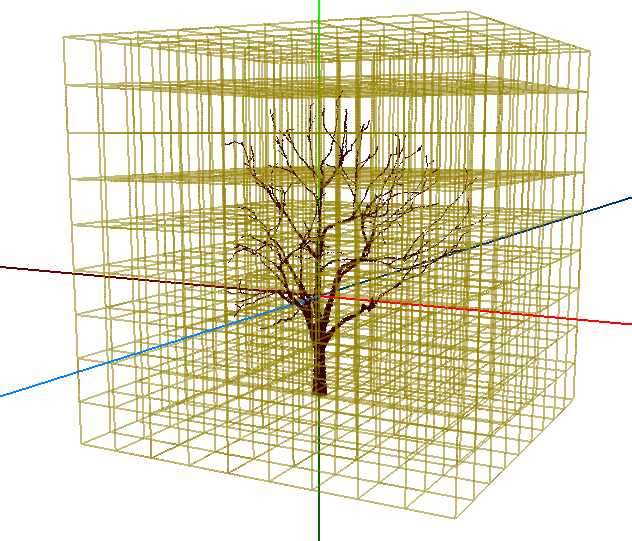
\includegraphics[height=8cm]{voxel.png}
	\caption{三维体素模型}
	\label{fig:voxel}
\end{figure}

\begin{algorithm}[H]
	\caption{点云模型体素化}
\begin{algorithmic}[1]
	\Require 点云模型$M$
	\Require 体素维度$d$
	\Ensure 三维体素数组$\mathbb{V}[1..d,1..d,1..d]$
	\State 初始化点云边界值$X_{max}=Y_{max}=Z_{max}=MIN\uline\quad FLOAT,X_{min}=Y_{min}=Z_{min}=MAX\uline\quad FLOAT$
	\ForAll{空间点$P(P_x,P_y,P_z) \in M$}
		\State $CheckBoundary(P)$
	\EndFor
\ForAll{空间点$P(P_x,P_y,P_z) \in M$}
\State $V_x = \frac{P_x-X_{min}}{X_{max}-X_{min}}\cdot d$
\State $V_y = \frac{P_y-Y_{min}}{Y_{max}-Y_{min}}\cdot d$
\State $V_z = \frac{P_z-Z_{min}}{Z_{max}-Z_{min}}\cdot d$
\State $\mathbb{V}[V_x, V_y, V_z] = \mathbb{V}[V_x, V_y, V_z] \bigcup \{P\} $
	\EndFor
\end{algorithmic}
\end{algorithm}

\subsection{三维体素泛洪确定邻域范围}
在确定了三维体素模型以后,便需要从根到叶,自底向上地对树的骨架结构进行生长。
生长的依据是已经得到的体素模型,将体素模型中点的分布作用于骨架的分支,便可以
张成骨架模型。

具体方法是将根节点置为当前节点,对其进行三维泛洪,首先对其相邻的27个体素进行泛洪,若
体素不为空,则将其加入邻域范围,若为空,则停止向该方向进行迭代。同时将加入邻域
范围的体素置为无效,表示其已经参与了泛洪,不再参与骨架的重建,这样不仅可以对算法
的结束有一个很好的约束条件,同时也可以减少重复处理的次数,加快算法的完成。然后进行下一次迭代,
对新加入的体素进行27方向的泛洪,并把有效的体素加入到邻域范围。接着比较两次迭代
体素增加的比例,如果低于设置的阈值,则停止迭代,当前的邻域范围即为三维泛洪得到
的当前节点的邻域范围。

图\ref{fig:3dfld}展示了三维体素泛洪确定邻域的步骤。\ref{fig:3dfld}(a)为其初始状态,
即邻域范围为当前体素。其中橙色的区域表示邻域范围,蓝色的区域表示未探索区域,灰色区域
表示空的体素,而绿色区域表示已经在之前的枝干邻域。\ref{fig:3dfld}(b)表示体素泛洪经过
一次迭代以后的状态,因为体素泛洪只会对与当前邻域范围相邻的未探索区域(蓝色方块)进行扩展,
所以\ref{fig:3dfld}(a)只会向黄色箭头指向的体素进行扩展,从而得到\ref{fig:3dfld}(b)。在得到
新的邻域后,首先会计算所新增的点的数量与之前的数量的比值有没有低于阈值,如果低于阈值,则停止
邻域的扩张。最后将得到\ref{fig:3dfld}(c)中的邻域范围。

\begin{figure}[H]
	\centering
	\subfloat[初始状态(邻域范围为1个体素)]{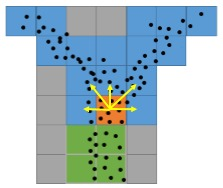
\includegraphics[height=3cm]{fld1.jpg}}\hspace{4em}
	\subfloat[第一次泛洪迭代(邻域范围为6个体素)]{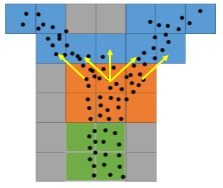
\includegraphics[height=3cm]{fld2.jpg}}\hspace{4em}
	\subfloat[第二次泛洪迭代(邻域范围为11个体素)]{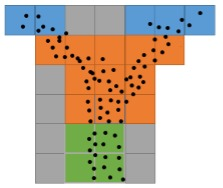
\includegraphics[height=3cm]{fld3.jpg}}
	\caption{体素泛洪示意图}
	\label{fig:3dfld}
\end{figure}

三维体素泛洪确定邻域范围算法的伪代码在算法表3中给出。
\begin{algorithm}[H] \label{alg:3dfld}
	\caption{三维体素泛洪确定邻域范围}
	\begin{algorithmic}[1]
		\Require 当前体素$C$,三维体素数组$\mathbb{V}[1..d,1..d,1..d]$,
		泛洪方向数组$\mathbb{D}[1..27]$,邻域范围增长比例阈值$\lambda$
		%\Require 三维体素数组$\mathbb{V}[1..d,1..d,1..d]$
		%\Require 泛洪方向数组$\mathbb{D}[1..27]$
		%\Require 邻域范围增长比例阈值$\lambda$
		\Ensure	邻域范围内体素集合$\mathbb{S}$
		\State 初始化单次迭代新增体素集合$\mathbb{S'}$
		\State $\mathbb{S'}.AddVoxel($根节点所在体素$)$
		\ForAll{泛洪方向$Direction \in \mathbb{D}$}
			\State $NewIndex = C.Index + Direction$
			\State $NewVoxel = \mathbb{V}[NewIndex.x,NewIndex.y,NewIndex.z]$
			\If{$NewVoxel$非空$\bigcap NewVoxel$有效}
				\State $\mathbb{S'}.AddVoxel(NewVoxel)$
			\EndIf
		\EndFor
		\State 体素增长比例$\mu=\frac{\mathbb{S'}.VoxelCount}{\mathbb{S}.VoxelCount}$
		\If{$\mu > \lambda$}
			\ForAll{$voxel \in \mathbb{S'}$}
				\State 把$voxel$作为当前体素进行递归调用
			\EndFor
		\EndIf
		\State \Return $\mathbb{S}$
	\end{algorithmic}
\end{algorithm}

在进行三维泛洪的时候,可以编程实现27个方向迭代过程的并行化,以提高算法的效率。

\subsection{通过最小二乘法线性拟合确定分支}
\label{subsec:leastsquares}
当得到邻域范围以后,便得到了邻域内体素在基于当前节点27个方向上的密度分布,而
每个体素内又包含着若干的点,因此等于是得到了在当前节点邻域内的点云分布情况。
接下来的工作就是怎样从各个方向的点云的分布情况抽取出核心的骨架。本文应用线性
拟合的方法来从密集的点中抽取出一条线段,作为该部分的骨架。

该方法首先要剔除掉那些点云密度很小的方向,以免每个节点都朝各个方向长出一些
细碎的枝条。因为这些细碎的枝条就算在此步中不剔除,到后续的轻量化的时候也不容许
它们的存在。

然后对于剩下的若干方向$d_1,d_2...d_k$,每个方向都对应着树木的一个骨架。在处理
某个方向$d_i$时,将其包含的体素中的所有点抽取出来,得到一个密集的点集$S_i$。
然后采用待定方程的办法,设直线方程为:
\begin{equation}
	\mathbf{x} = \mathbf{x_0} + \mathbf{d}t,\quad(t \in [0,\infty))
\end{equation}

其中$\mathbf{x_0}$是当前节点的坐标,$\mathbf{d}$是待拟合的直线方向。我们假设
点集$S_i$中的点$P_1,P_2,...P_m$都在直线上,则可以得到以下方程组:\\

\begin{equation} \label{eq:line}
	\left\{ 
		\begin{array}{lll}
			a_{11}d_x+a_{12}d_y+a_{13}d_z & = & b1\\
			a_{21}d_x+a_{22}d_y+a_{23}d_z & = & b2\\
			... & & \\
			a_{n1}d_x+a_{n2}d_y+a_{n3}d_z & = & bn
		\end{array}
	\right.
\end{equation}

其中具体数值未给出,注意这里的$n=3m$,因为每个点$P$可以提供三个方向的方程式。
在这个方程组中,令\\
\begin{displaymath}
	\mathbf{U}=
\left(
\begin{array}{ccc}
	a_{11} & a_{12} & a_{13}\\
	a_{21} & a_{22} & a_{23}\\
	... & ... & ...\\
	a_{n1} & a_{n2} & a_{n3}\\
\end{array}
\right)
,\quad
\mathbf{d}=
\left(
\begin{array}{c}
	d_x\\
	d_y\\
	d_z
\end{array}
\right)
,\quad
\mathbf{b}=
\left(
\begin{array}{c}
	b_1\\
	b_2\\
	...\\
	b_n
\end{array}
\right)
\end{displaymath}


在实践中,由于筛选方向上的点数较多且发散分布,由线性代数的理论知,$\mathbf{U}$是过约束的,
即$n>r$,其中$r$是矩阵$\mathbf{U}$的秩。这种情况下没有标准的解,只能找到使误差最小的向量$\mathbf{d}$,
误差定义为:\\
\begin{equation}
	E\xlongequal{def} \sum_{i=1}^n(\mathbf{d}t_i - \mathbf{x_i} + \mathbf{x_0})^2=|\mathbf{Ud}-\mathbf{b}|^2
\end{equation}

由于$E$正比于方程的均方误差,因此只要E达到最小值,那么点集相对于该直线的波动就最
小。换句话说,也就是该直线最好的模拟了该点集所表示的骨架。由线性代数的方法很容易
可以解得$\mathbf{d}=\mathbf{[(U^TU)^{-1}U^T]b}$。图\ref{fig:fitting}展示了由当前
节点(蓝色节点)分别向两个点云集合拟合出的两条直线(红色线段),这两条直线将被作为两个
分支的方向。从图中可以看出线性拟合的方法可以很好的估计出树木分枝的方向,从而准确的
恢复出树木的父子结构。

\begin{figure}[H]
	\centering
	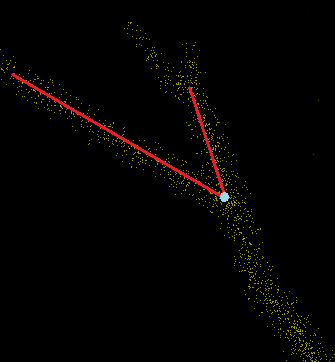
\includegraphics{fitting.png}
	\caption{线性拟合计算分支方向}
	\label{fig:fitting}
\end{figure}

算法表4中给出了得到邻域信息后进行骨架抽取的伪代码,其中\textit{Least Squares Processing}表示运用最小二乘法进行
线性拟合。

\begin{algorithm}[H]
	\caption{基于邻域的骨架抽取}
	\begin{algorithmic}[1]
		\Require 当前节点体素$V$
		\Require 骨架方向数组$\mathbb{D}[1..n]$
		\Ensure 当前节点子节点集合$\mathbb{S}$
		\ForAll{骨架方向$d\in D$}
			\State $NewChild\gets Least Squares Processing$
			\State $\mathbb{S}.AddChild(NewChild)$
		\EndFor
		\State \Return $\mathbb{S}$
	\end{algorithmic}
\end{algorithm}

\subsection{获取骨架半径}
树木骨架的半径对树木模型的真实感有着十分显著的贡献,所以尽可能准确的获得骨架的
半径信息能够有助于重建出极具真实感的树木模型。对于树木半径的获取方法也有许多,
主要分为根据规则生成半径和从树木点云结构中获取半径两种方式。

对于基于规则来生成半径,最简单的方法是对树木半径进行线性地递减,即$r=cR$,其中
$r$为子枝半径,$R$是父枝半径,$c$为一个线性倍数,这个倍数可以固定,也可以进行
随机的扰动从而增进多样性。Leonardo da Vinci在经过大量观察后总结出了一种更符合自然规律
的树木父子枝直径的关系公式:$D^2=\sum_{i=1}^n{d_i^2}$,其中$D$为父枝直径,$d_i$为第
$i$个子枝的直径,$n$为子枝的数量。这个公式被广泛地用于树木枝干的半径模拟。

区别于基于规则的半径生成方法,本文为了进一步提升真实感,选择在进行骨架抽取的同时,
同样进行半径抽取的方法。注意,用该方法的前提是点云分布须均匀化,然而基于图像进行三维重建
得到的树木点云会呈现表皮化的现象,这是由于图片上的点都是树木的表皮点,所以在得到
三维点云后,是需要进行一些修复工作的,本文用随机点填充的方法对该点云模型进行了实心化
的修复。当点云分布满足均匀化时,在对某个骨架进行拟合之后,对于拟合出来的直线,来计算
所有参加拟合该直线的点到该直线的平均距离$D_{avg}$,然后就可以计算该骨架的半径$R=D_{avg}*2$。
由于点云分布均匀,所以半径显然就是平均距离的2倍。该算法的伪代码在算法表5中给出。\\

\begin{algorithm}[H]
	\caption{骨架半径抽取}
	\begin{algorithmic}[1]
		\Require 拟合出的当前骨架直线$L$
		\Require 当前骨架的点集$\mathbb{S}$
		\Ensure 当前骨架半径$R$
		\State 初始化距离和$D_{sum}=0$
		\ForAll{空间点$P \in \mathbb{S}$}
		\State 点到直线距离$D_{sum}+=CalculateDistance(P, L)$
		\EndFor
		\State 平均距离$D_{avg}=D_{sum}/\mathbb{S}.Count$
		\State 骨架半径$R=D_{avg}*2$
		\State \Return $R$
	\end{algorithmic}
\end{algorithm}

图\ref{fig:radius}给出了三种半径求解方法的效果对比。\ref{fig:radius}(a)给出了线性衰减方法
的结果,该方法中子枝半径以父枝半径的线性倍衰减。\ref{fig:radius}(b)给出了前文提到的Leonardo
 da Vinci规则所生成的半径情况。\ref{fig:radius}(c)则采用本文中基于线性拟合直线,再计算所有点
 到该直线平均距离的方法。从三者的效果中可以看出,线性衰减容易出现部分枝条生长不自然的现象,究其
 原因,还是因为一个单一的绝对的线性系数无法适用于所有的枝条,它对于某些枝条会偏大,对于另外一些
 枝条会偏小。 Leonardo规则虽然给出的是一种父子枝之间的相对关系,从一定程度上解决了线性系数单一
 绝对而导致的问题,但是它生成的树木枝干会出现过于均与化,而没有捕捉到现实中树木各个局部的特征。
 本文的方法则由于其基于对所有点的实际恢复坐标进行统计,而更加注重树木的实际局部特征情况,
 其效果也是三者之中最好的。
 \begin{figure}[H]
	\centering
	\subfloat[样本图像]{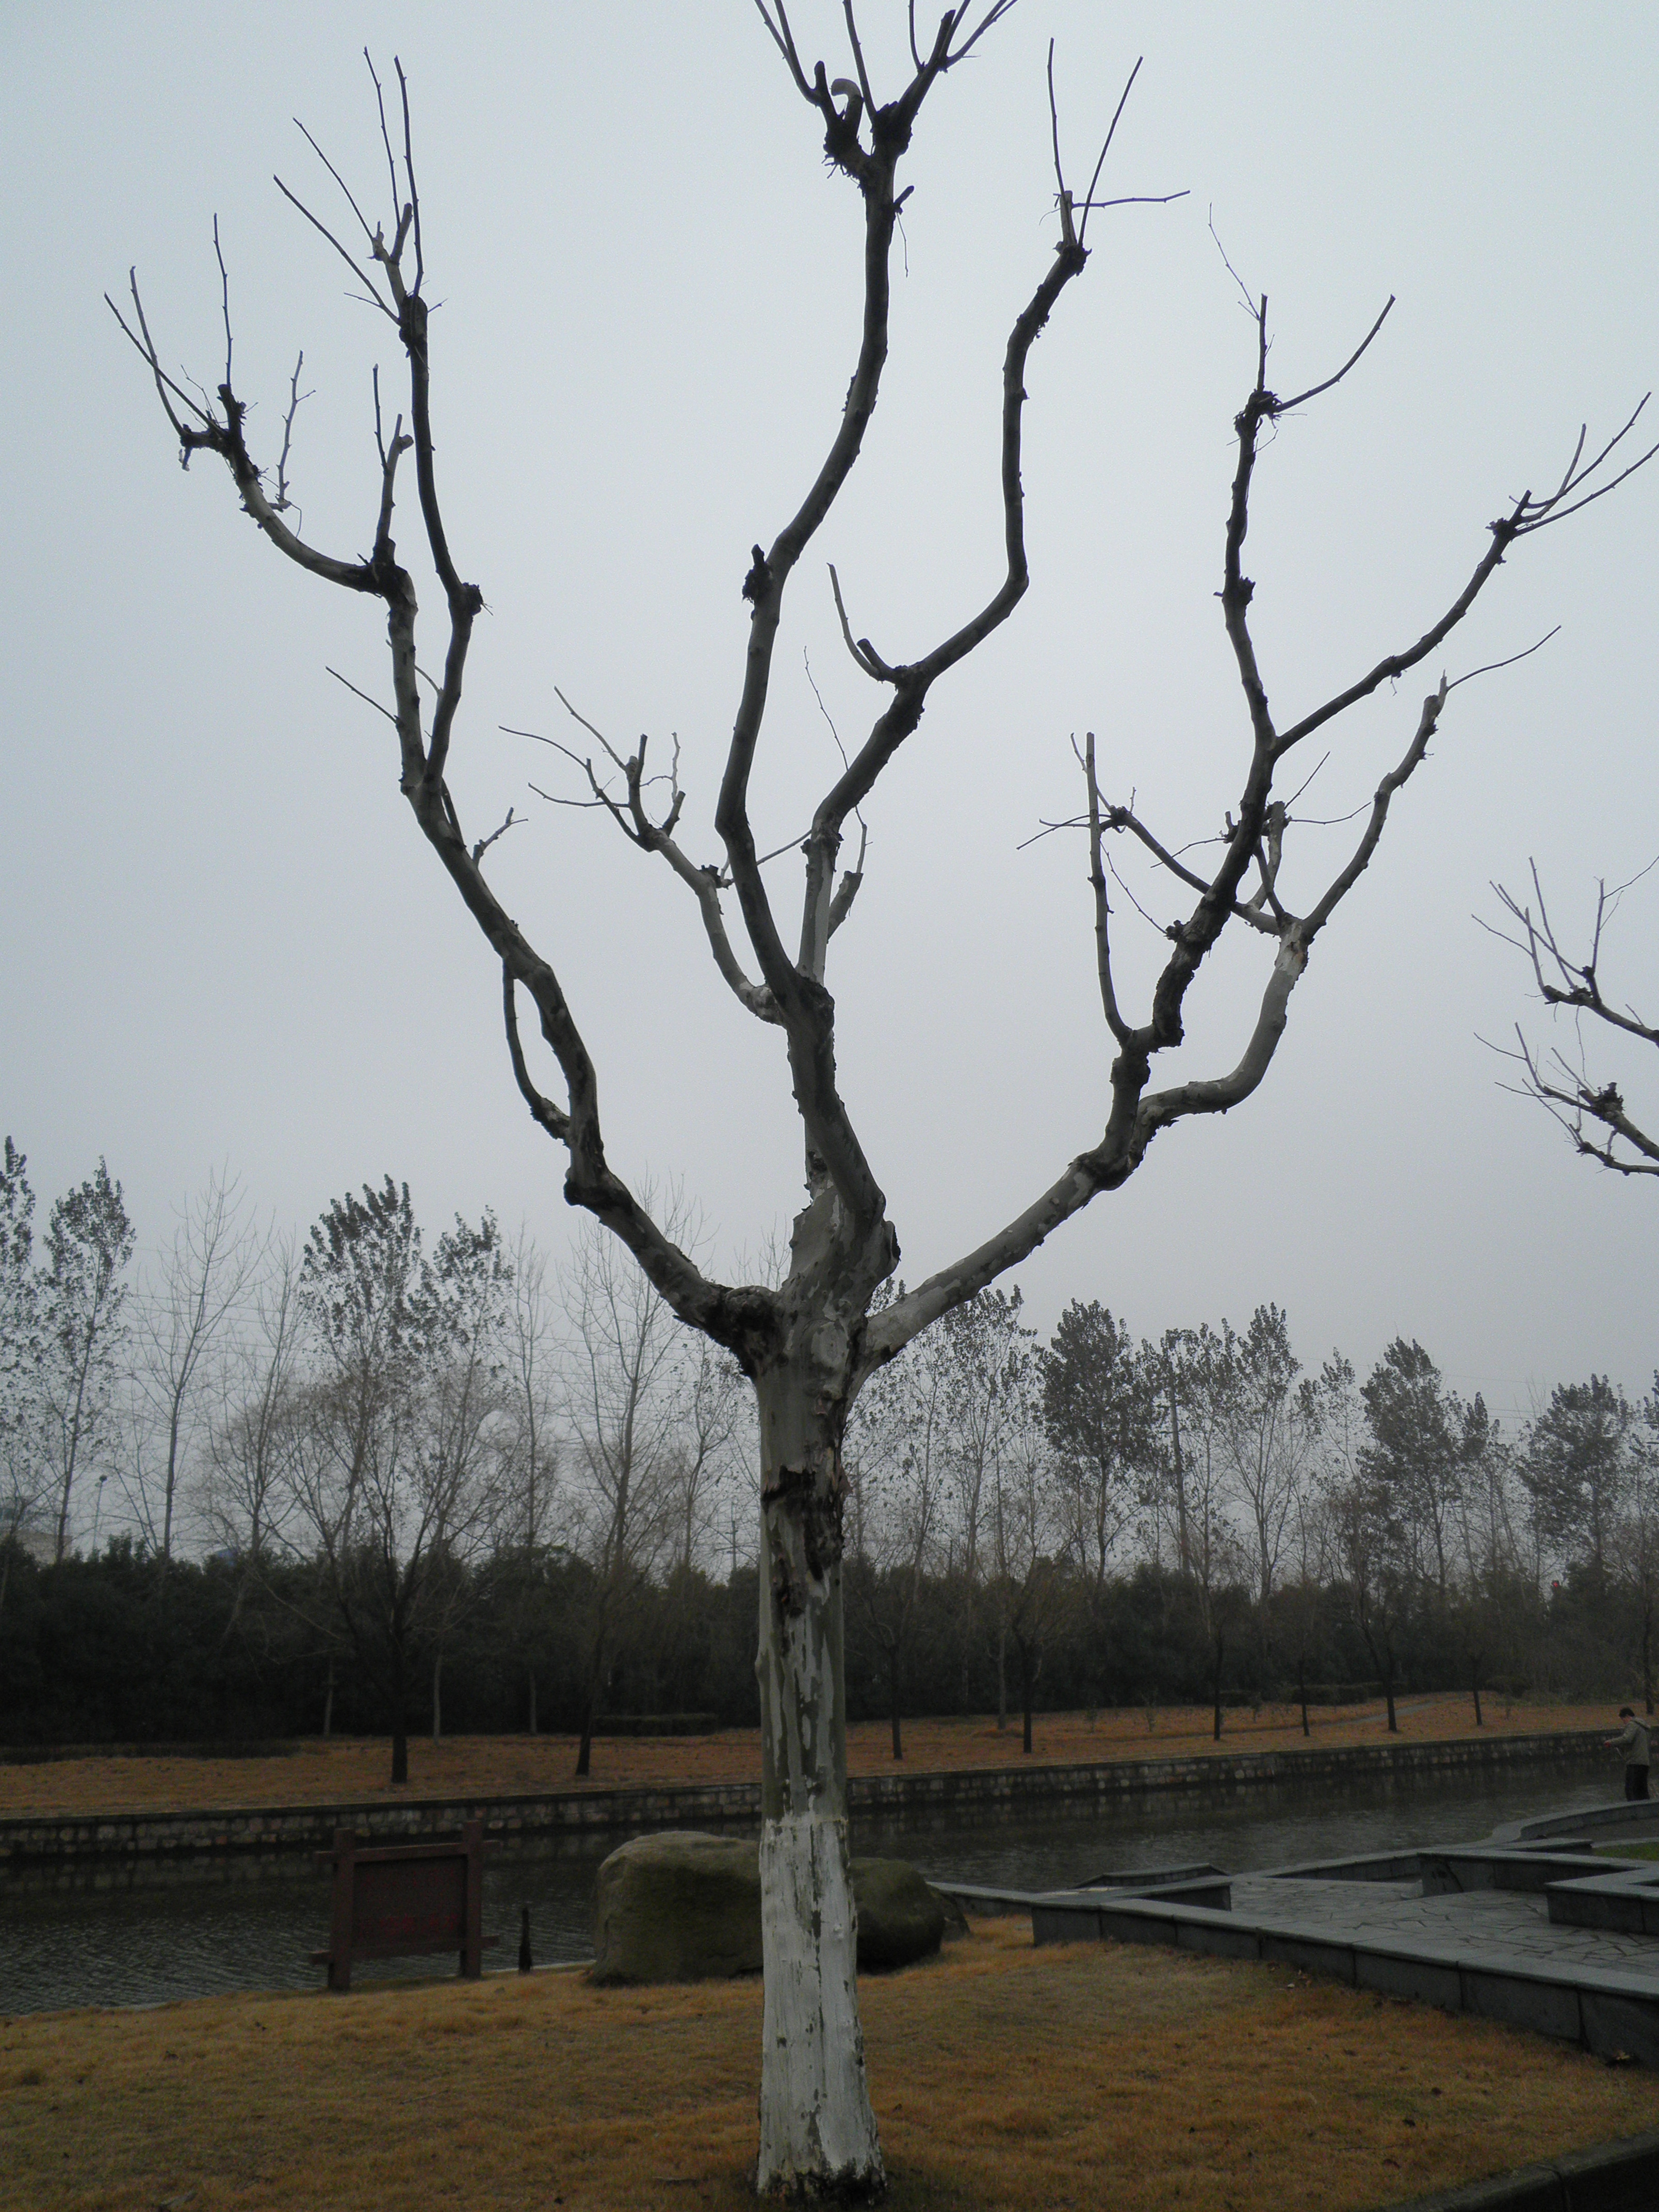
\includegraphics[height=6cm]{rsample.jpg}}\hspace{4em}
	\subfloat[线性衰减]{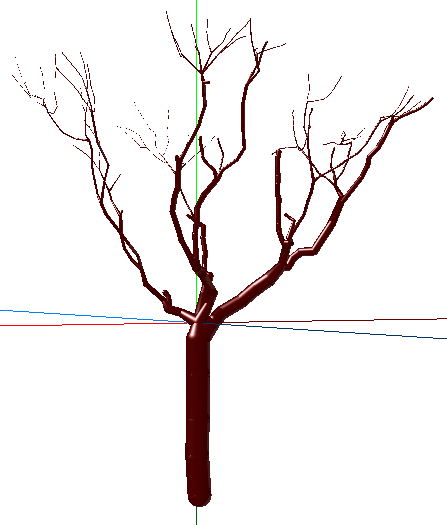
\includegraphics[height=6cm]{rlinear.png}}\hspace{4em}
	\subfloat[Leonardo规则生成]{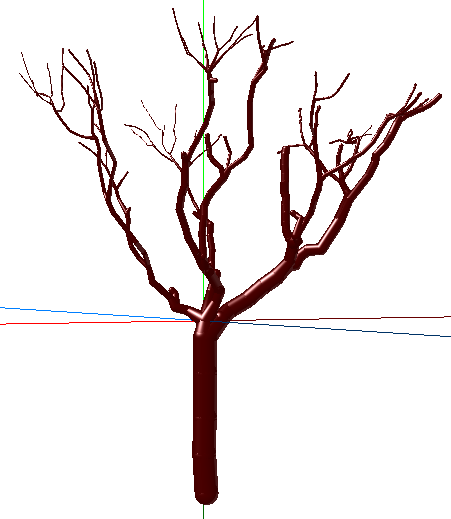
\includegraphics[height=6cm]{rsquare.png}}\hspace{4em}
	\subfloat[基于拟合的半径抽取]{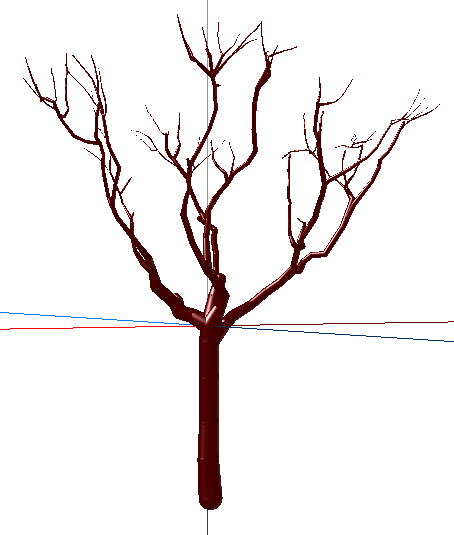
\includegraphics[height=6cm]{raffine.png}}\hspace{4em}
	\caption{三种计算半径方法效果对比}
	\label{fig:radius}
\end{figure}

%---------------------------------轻量化-----------------------------------
\section{基于枝干合并的轻量化处理}
\label{sec:branchcombine}
用基于多方向迭代与步长探索得到的三维树木骨架通常是很细致和准确的,尽管它相对于
用3DSMAX等建模工具手工建模得到的面片模型已经大大的轻量化了。但是如果应用是用于
大规模的树木建模,那么我们有必要根据应用需求进一步进行轻量化处理。

\subsection{L-System的尝试}
\label{subsec:lsystem}

\subsubsection{L-System简介}
L-System是一种并行的重写系统和正规语法,
它的结构可以用可以定义为一个3元组:\\
\[\mathbf{M} = (V, \omega, P)\]
其中:\\
\begin{itemize}
	\item $\mathbf{V}$(字母表) 表示可以被替代的字符的集合。
	\item $\mathbf{\omega}$(初始串) 表示L-System的初始状态。
	\item $\mathbf{P}$(规则集合) 表示一系列的衍生规则。
\end{itemize}
L-System可以根据这三个组成部分的不同而递归地产生形态各异的字符串。
由于L-System具有递归生长的特性,因此我们可以用L-System规则来表达一个具有自相似形态
或者分形结构的物体,比如本文所研究的对象\raisebox{0.5mm}{------}树木。

\subsubsection{树木模型的参数化L-System规则抽取}
球面海龟几何的提出,用参数化的L-System规则描述了树木的结构信息。在球面海龟几何中,
节点的空间几何信息用4个量(长度$l$、半径$r$、父子枝夹角$\theta$和水平转角$\phi$)
和4个扩展符号(+、-、\&、$\wedge$)来表示:
\begin{itemize}
	\item $+(l)$	表示以当前位置为起点,在当前方向上前进$l$单位个长度
	\item $!(r)$	表示设置当前节点半径为$r$
	\item $\&(\theta)$	表示设置父子枝夹角为$\theta$
	\item $\wedge(\phi)$	设置水平偏角为$\phi$
\end{itemize}
在球面海龟几何中,将每个骨架节点生成一条参数化的L-System规则,形如:\\
\begin{equation} \label{eq:turtle}
N(l,r) \rightarrow \&(\theta_0)\wedge(\phi_0)!(r) + (l)S_0(l*a_0,r*b_0)...\&(\theta_n)\wedge(\phi_n)!(r) + (l)S_n(l*a_n,r*b_n)
\end{equation}

其中N表示当前枝条,$S_0~S_n$表示当前枝条的n个子枝条,$a_i和b_i$分别表示第i个子枝条
与当前枝条的长度比和半径比,$\theta_i和\phi_i$分别表示第i个子枝条与当前枝条的空间
夹角和水平偏角。

\subsubsection{使用L-System进行树木轻量化建模遇到的问题}
在用参数化L-System进行树木轻量化建模时,在进行规则归纳时,有个难以克服的问题。考虑
将规则\ref{eq:turtle}中的$a_0$换成$a_0'$,则规则变成一个完全不同的规则。这意味着对于
两个分支规则,这两个规则中的子枝的长度,半径,转交,偏角等必须完全相等才能归纳为同
一个规则。而对于自然界中形态结构复杂的树木,每个分支规则几乎不可能完全等同于另一个
规则。

对上面的问题有一种解决方法就是将参数区间化,将属于同一区间的参数的值视为相同。比如
我们可以将父子枝间的转角分为18个区间,每个区间的大小为10度。但是经过分析就可以察觉,
这并没有从根本上解决这个问题。假设我们将这4个变量都各自划分为10个区间,那么规则总数
最多可以有10000个,而且在这种情况下,两个规律相同的几率也是非常小的。如果我们将分区
数量减少,则又有可能将本来差异比较大的规则归纳为一个规则,不符合真实感的要求。

所以,经过分析,这种用参数化L-System进行树木轻量化建模的方法并不适用于从骨架中去抽取
规则,而是适用于反向地用其描述的规则去产生一棵树,如台湾学者戴文凯就对单棵树的L-System
规则进行随机扰动而轻量化的建模出了整片森林。

\subsection{树木轻量化?枝干合并!}
\label{subsec:branchmerge}
用L-System的方法抽取规则所产生的问题,从本质上看,是由于自然界中的树木形态太复杂和多变。
与其从一个本就不规则生长的事物中去抽取规则,还不如直接地在其逻辑结构上进行一系列的轻量
化操作。本文提出了对已抽取的树木骨架中对视觉影响不大的部分进行合并的方法,从而在尽可能
保证模型的视觉效果的基础上,进一步地减小树木模型的体积,使得其能更广泛地应用到WebVR、WebGame
等各个领域。

树枝的结构其实只由核心的一些枝干组成,其他的枝干只是对其结构进行微调。所以在要求进一步轻量化
的前提下,本文提出了分别从纵向和横向对树枝进行合并的方法,以去掉一些只是起到微调作用的枝干。
这种方法在尽可能保证真实感不过多丢失的前提下对树枝进行简化操作,以适应更广泛的Web应用领域。

纵向合并表示从父到子,从根到页进行纵向递归式的合并。若当前节点与其父节点和子节点的夹角小于所设定
的阈值,那么则将该节点去掉,并将其子节点连接到其父节点。注意,若该节点的子节点数目不只一个,
那么我们不对它进行合并操作,因为将该节点的所有子节点加到该节点的父节点上去有违真实感。
图\ref{fig:vert}展示了树枝纵向合并过程。图\ref{fig:vert}(a)为输入的树枝骨架,并且当前节点
为\textbf{B},其父节点为\textbf{A},且只有唯一的子节点\textbf{C}。设合并角度阈值为$\alpha$,
假设\textbf{AB,BC}之间的夹角b小于合并阈值$\alpha$,那么将\textbf{B}剔除,并将\textbf{C}作为
\textbf{A}的子节点。同理,在图\ref{fig:vert}(b)中,若夹角c小于阈值$\alpha$,那么也将\textbf{AC}
和\textbf{CD}合并。在图\ref{fig:vert}(c)中,由于节点\textbf{D}有两个孩子,所以不对其进行合并
操作。

纵向合并算法的伪代码在算法表6中给出。

\begin{figure}[H]
	\centering
	\subfloat[输入树枝骨架]{
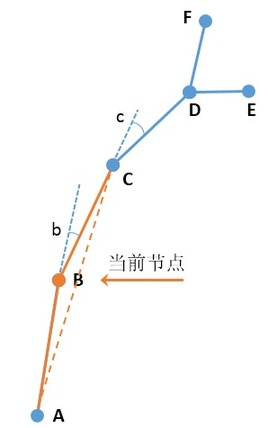
\includegraphics[height=5cm]{vert1.jpg}}
\hspace{4em}
	\subfloat[合并AB、BC]{
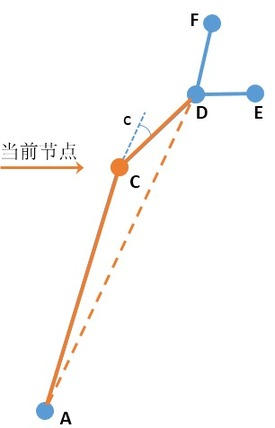
\includegraphics[height=5cm]{vert2.jpg}}
\hspace{4em}
	\subfloat[合并AC、CD]{
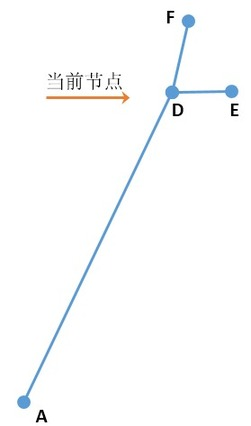
\includegraphics[height=5cm]{vert3.jpg}}
	\caption{树枝简化过程}
	\label{fig:vert}
\end{figure}

\begin{algorithm}[H]
	\caption{纵向合并枝干}
	\begin{algorithmic}[1]
		%\Comment {根据纵向合并角度参数,以当前节点为发起点递归式地纵向合并枝干}
		\Require 纵向合并角度$\alpha$
		\Require 当前节点$N$
		\Ensure None
		\ForAll{节点$N'\in N.Children$}
		\While{$N'.ChildCount = 1$}
		\State $\vec{u} \gets N'.Position-N.Position$
		\State $\vec{v} \gets N''.Position-N'.Position$
		\State $\gamma \gets \cos^{-1}({\frac{\vec{u} \cdot \vec{v}}{|\vec{u}|\cdot|\vec{v}|}})$
		\If{$\gamma<\alpha$}
		\State $N.child \gets N.AddChild(N'')$
		\State $N.child \gets N.DeleteChild(N') $
		\EndIf
		\State $N' \gets N'.FirstChild$
		\EndWhile
		\EndFor
		\If{$N.ChildCount > 1$}
		\ForAll{节点$N'\in N.Children$}
		\State 以$N'$为当前节点递归调用该函数
		\EndFor
		\EndIf
	\end{algorithmic}
\end{algorithm}

横向合并指的是对叶子节点和与其夹角小于阈值的兄弟节点进行合并。之所以只对叶子节点进行合并,是
因为非叶子节点下面都有若干棵子树,若对它们进行合并,必须对它们下面的子树也进行合并。而合并子树
显然就使得真实感下降很大,因为这不只是局部微调,而是若干子树的变动。横向合并的伪代码在算法表7中
给出。

\begin{algorithm}[H]
	\caption{横向合并枝干}
\begin{algorithmic}[1]
	\Require 初始化横向合并角度$\beta$
	\Require 设定当前节点$N$
	\Ensure None
	\ForAll{节点对$P\in N.Children$}
		\State $N_1 \gets P.FirstNode$
		\State $N_2 \gets P.SecondNode$
		\If{$N_1.ChildCount = 0 \wedge N_2.ChildCount = 0$}
			\State $\vec{u} \gets N_1.Position - N.Position$
			\State $\vec{v} \gets N_2.Position - N.Position$
			\State $\gamma \gets \cos^{-1}({\frac{\vec{u} \cdot \vec{v}}{|\vec{u}|\cdot|\vec{v}|}})$
			\If{$\gamma<\beta$}
				\State $New\ Node\ N'$
				\State $N'.Position \gets (N_1.Position+N_2.Position)/2$
				\State $N'.Radius \gets max(N_1.Radius,N_2.Radius)$
				\State $N.child \gets N.DeleteChild(N_1)$
				\State $N.child \gets N.DeleteChild(N_2)$
				\State $N.child \gets N.AddChild(N')$
				\State 退出循环并以当前节点N重新调用该函数
			\EndIf
		\EndIf
	\EndFor
	\ForAll{节点$P\in N.Children$}
		\State 以P为当前节点递归调用该函数
	\EndFor
\end{algorithmic}
\end{algorithm}

纵向合并和横向合并单独使用时都具有很大的局限性,因为纵向合并只能对具有单个孩子并且没有
兄弟的节点进行纵向递归地调用,而横向合并又只能对叶子节点进行兄弟级别的合并。但是将两种
合并方法联合使用,将可以从整体上对树木进行微调操作,图\ref{fig:combine}对这一想法进行了
演示。\ref{fig:combine}(a)中经过纵向的\textbf{AC,CD}合并得到\ref{fig:combine}(b)。
\ref{fig:combine}(b)中由于\textbf{D}有两个子节点,无法进行纵向合并,所以考虑进行横向
合并\textbf{DE,DF},并得到\ref{fig:combine}(c)。最后进行一次纵向合并得到\ref{fig:combine}(d)。

\begin{figure}[H]
	\centering
	\subfloat[输入枝干骨架]{
	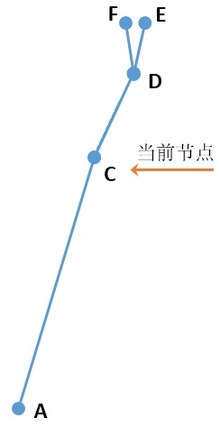
\includegraphics[height=3cm]{comb1.jpg}}
	\hspace{4em}
	\subfloat[纵向合并AC,CD]{
	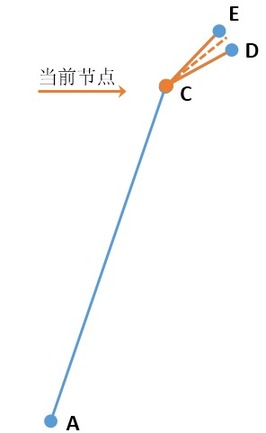
\includegraphics[height=3cm]{comb2.jpg}}
	\hspace{4em}
	\subfloat[横向合并DE,DF]{
	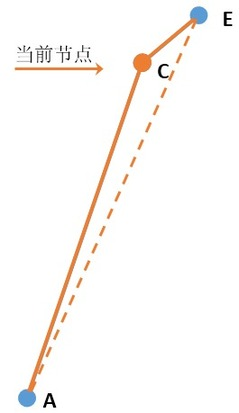
\includegraphics[height=3cm]{comb3.jpg}}
	\hspace{4em}
	\subfloat[纵向合并AD,DE]{
	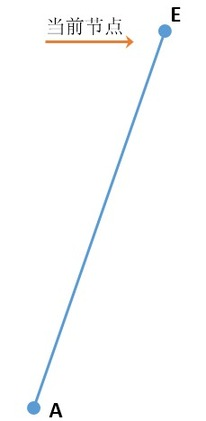
\includegraphics[height=3cm]{comb4.jpg}}
	\caption{联合使用纵向和横向合并}
	\label{fig:combine}
\end{figure}

%---------------------------------质量评估----------------------------------
\section{建模还原度}
\label{sec:qualityevaluation}
对于一个通过建模获得的树木模型,如果没有一个客观的量化评价指标,就无法从客观的角度
反馈树木模型的还原度和各个步骤算法的可行性。对于本文的基于图像序列的树木建模方法,
建模的输入是在自然环境下拍摄的树木图片序列,输出是三维的骨架模型。因此,判断三维模型
和投影照片的相似程度是评价建模质量的核心。然而,大多数基于图像的树木建模论文\cite{quanlong,
tanping,lichuan,tanping2,liu}只给出了输入图片和建模结果在少量角度的渲染效果,试图让
观察者从肉眼观察其相似度。但是这种方法是主观的,因观察者的不同可能会有不同的评价结果,
这显然不是一个好的评价方法。

为了客观、量化地评价基于图像序列的建模质量,本文提出了一套完整的评价方法。然而,仅仅凭借照片
无法完全表达出其所在环境的信息,比如环境光照,因为遮挡而产生的阴影信息等,因此本文的评价
方法将不针对模型的纹理和颜色信息,仅仅对模型的几何信息和照片中的几何信息的匹配程度进行量化
分析。

设树木模型$M$由$n$张从不同角度拍摄的同一棵树的图片序列$I_1\sim I_n$,经过基于图像的三维重建,
骨架抽取的方法进行建模所获得。那么模型$M$的建模还原度$\mathbb{Q}$定义如下:\\
\begin{definition}
	\[\mathbb{Q}=\mathbf{I}\cdot\mathbf{R_{3d}}\cdot\mathbf{R_s}\]
\end{definition}

建模还原度$\mathbb{Q}$的取值范围为$[0,1]$,0表示没有还原出任何树木几何信息,1表示准确还原出
整棵树木的几何信息。

本文将建模还原度$\mathbb{Q}$考虑由3个部分组成,为此也引入了三个新的概念:图片序列信息量$\mathbf{I}$,
三维重建还原度$\mathbf{R_{3d}}$,以及骨架抽取还原度$\mathbf{R_s}$。这三个分量的取值范围都为$[0,1]$,它们
的乘积即为总的建模还原度$\mathbb{Q}$。后续小节会详述这三个分量。

\subsection{图像序列信息量}
当实地对树木进行多角度拍摄时,拍摄者将基于不同的水平角度对树木进行全方位的拍摄,以便将整棵树的
信息尽可能多的携带进图像序列中。然而,从客观上来看,怎么样的图片序列才更加完整的表达了整棵树的
几何特征?为了从客观和量化的角度给出树木图像序列所携带的树木信息的多少,本文引入了图像序列信息量的概念。

那么,到底怎样的图片序列携带的信息量更大呢?从拍摄过程分析,如果想要得到一棵完整的树木信息,那么
需要绕着一棵树一圈进行密集地拍摄。这里的一圈,用数学化的表示,就是$360^\circ$,如果只是绕半圈进行
拍摄,那么所得到的图片序列表达的树木信息必定是不完整的,所以角度对信息量有着很大的贡献。另一方面,
如果每隔$60^\circ$进行一次拍摄,和每隔$30^\circ$进行一次拍摄,在它们都绕圈拍摄的前提下,后者的图片序列所
含信息量必然更大。再进一步思考,如果我隔$360^\circ,180^\circ,90^\circ,..., 1^\circ$进行拍摄呢?那么后一次拍摄所得的图
片序列相比前一次的图片序列信息量的增长是相同的吗?答案是否定的,因为当图片很少时,三维重建的结果也不好,
这时增加图片数量是能够很大程度上改观三维重建的重量的,因此此时的信息量增长速度快。
但是在拍摄已经比较密集的情况下,后一次拍摄所增加的信息量必定只是一些细节的信息,所以,信息量增长的速率应该变小。
并且一个信息量大的图片序列应该满足以下三个要求:\\
\begin{itemize}
	\item \textbf{图片数量多}: 图片数量多也就意味着拍摄角度多,因为一张图片代表着一个角度。
	\item \textbf{角度跨度大}: 跨度大指需要对树木进行全方位的拍摄。
	\item \textbf{角度分布均匀}: 若图片只是密集的集中在一个角度区间,就算图片再多,也无法完整地表达整
								  棵树的信息,所以若在角度多和跨度大的情况下还满足分布均匀,那么就能很完整
								  地携带树木的信息。
\end{itemize}

由于从平面的2D图像很难得到其空间角度拍摄情况,因此在这里我们简化其定义,将关注点放在图片数量上来,对于
图片跨度和角度的均匀分布,我们默认拍摄者在拍摄过程中采用均匀的角度偏差来进行$360^\circ$的拍摄。

根据以上的分析,本文给出了图像序列信息量的数学定义如下:\\
\begin{definition}
	\[ \mathbf{I}=1-(\frac{a}{b})^n \]
\end{definition}

其中,图片序列信息量$\mathbf{I}$的取值范围为$[0,1]$。当$\mathbf{I}=0$时表示图片序列并不包含树木信息,
当$\mathbf{I}=1$时表示图片序列能完全表达空间树木的几何信息。$a,b$都是正数且$a<b$,具体数值需要对不同树木
进行实验之后才能得到。尽管$a$和$b$因树木特点不同而不同,但是它始终满足前文提出的信息量增长速度的特点,
即先快后慢。

\subsection{三维重建还原度}
对于一个给定的图片序列,所用三维重建方法所得到的点云模型的与实际的树木在几何形状上的相似度如何,由三维重建
还原度$\mathbf{R_{3d}}$来定义。注意,实际树木的几何信息被记录在输入的图像序列中,所以想要计算点云模型和实际树木
的相似度,就需要对点云模型和图片序列进行比较。然而对于三维的点云信息和二维的图片信息,无法进行直接地比较。一个
比较直观的想法,是对三维的点云进行投影,投影的角度由三维重建过程中的照相机几何标定步骤给出。

由于不考虑模型纹理和颜色信息,在空间点被投影到平面以后,只关注其是否在对应角度图片的树木轮廓内。所以对输入的树木
图片序列,需要先获得其轮廓图,并将其转化为二值图像。树木上的点值为1,而树木外的点值为0。对于每一个点云模型中的点,
按对应角度投影,获得其在对应图片上的坐标值,并且在其二值图像上确定其值,若为1,则表明匹配成功,否则匹配失败。最后
统计出匹配成功的总的比例,作为三维重建的还原度。

根据以上分析,本文给出三维重建还原度的数学定义式:\\
\begin{definition}
	\[ \mathbf{R_{3d}}=\frac{1}{n}\sum_{i=1}^n \frac{P_i}{P_i+O_i}\]
\end{definition}

上式中的$n$表示图像的数量,$P_i$表示点云模型投影到第$i$张图片上在树木轮廓中的点的数量,$O_i$表示点云模型投影到第
$i$张图像上在树木轮廓外的点的数量,因此$P_i+O_i$自然就表示点云模型中点的总数量。$\frac{P_i}{P_i+O_i}$表示点云投影到
第i张图片上的击中率。最后对每张图像的击中率求平均,作为总的三维重建的还原度。其值区间为$[0,1]$。

\subsection{骨架抽取还原度}
骨架抽取是基于三维点云模型进行的,因此计算骨架抽取的还原度的输入是重建出的点云模型和抽取出的骨架模型。由于点云模型是
三维的点的集合,而抽取出的骨架模型却是一个记录着树形结构的逻辑信息,它们无法进行直接的比较。本文采取的做法是将骨架的
树形逻辑信息用圆台和球进行堆叠从而将其转化为三维的表示。

具体的做法是对骨架中的每个节点,根据其半径构造出一个球体。然后对于每个父子关系,用一个圆台来表示其枝干,圆台的底半径
等于父节点的半径,圆台的顶半径等于子节点的半径。然后对于每个点云模型中的点,用数学公式判断其是否存在于骨架的三维表示中
的球体或圆台中,如果存在,则表示匹配成功,否则表示匹配失败。最后用成功点数与总点数的比值来表示骨架抽取的还原度。定义如下:\\
\begin{definition}
	\[ \mathbf{R_s}=\frac{S}{N} \]
\end{definition}

其中$S$表示匹配成功的点数,而$N$表示点云模型的总点数。$\mathbf{R_s}$的值区间为$[0,1]$。

注意,若用经过枝干合并轻量化处理的骨架进行骨架抽取还原度计算,其值必定会比直接从点云中抽取出来的模型要小,因为模型经过
简化后,与原点云模型的匹配度也必将降低。本文的目标只是尽可能在还原度降低不多的情况下,对骨架进行尽可能多的轻量化。

\subsection{建模还原度计算}
将图片序列信息量$\mathbf{I}$、三维重建还原度$\mathbf{R_{3d}}$和骨架抽取还原度$\mathbf{R_s}$代入建模还原度$\mathbb{Q}$
的定义式中,可以得到建模还原度的计算式:\\
\begin{equation}
	\mathbb{Q}= (1-(\frac{a}{b})^n)\cdot \frac{1}{n}\sum_{i=1}^n \frac{P_i}{P_i+O_i} \cdot \frac{S}{N}
\end{equation}

\section{本章小节}
\label{sec:conclusion}
本章具体阐述了基于图像树木轻量化建模所涉及的一些算法。

首先介绍了光流法的由来,并且分析了LK光流法的思想和特点,然后介绍了基于图像金字塔的PyrLK光流法,这种方法用图像金字塔这种多
分辨率图像层来克服图像中的大块运动,是LK光流法的一种优化与实现。接着提出了改进的PyrLK光流法,该算法把PyrLK的局部平移假设
扩展到了局部仿射变换假设,并且加入了特征反向追踪,以提高算法鲁棒性,实现了高精度的匹配。

三维体素泛洪是计算机图形学中二维像素泛洪的扩展,它将三维体素按洪水泛滥一般进行空间的扩展。本文利用三维体素泛洪实现了节点
对邻域的探索,并在该邻域的范围内对方向进行分割,将每个分割方向上的点集根据最小二乘法进行拟合,得出该方向上骨架具体的直线方程。
然后根据点集内点到对应直线方程的距离大小,算出该骨架的半径大小。从而得到具有半径信息的骨架结构。

在得到骨架结构后,为了迎合轻量化的应用,本文对其进行轻量化操作。本文首先对传统的轻量化方法L-System进行了尝试,运用参数化
的L-System规则进行规则抽取,但是由于现实中树木的复杂性与不规则性,抽取出来的规则太多,以至于违背了轻量化的原则。于是本文
提出了基于枝干合并的轻量化方法,分别从纵向和横向对树木枝干进行合并,以达到轻量化的目标。

本章的最后,本文还提出了基于图像树木轻量化建模的质量评价方法。提出了建模还原度的概念,它包含了三个子项:图像序列信息量、
三维重建还原度以及骨架抽取还原度。它们分别代表了图像序列对真实树木的信息携带量、点云模型和图像序列的匹配度和骨架模型与点云模型的匹配度。
本文对这三个子项的由来和计算方法都进行了阐述,并将它们融合给出了建模还原度的计算式。

\chapter{基于三维体素泛洪与线性拟合的三维树木骨架抽取}
\label{sec:sklextract}
在获取了精确的点云模型之后,出于后续轻量化的考虑,需要将模型的存储方式由
密集的点云转化为逻辑的父子结构。用树形的数据结构来表达现实的树结构,这是很
自然的想法,相对于面片结构,树形结构也是一种更为轻量化的存储方式。每个节点表示
树枝的起点,存储着该节点的空间位置,半径和该节点的父子枝信息以及兄弟信息。一个
节点和它的一个子节点形成一个空间线段,若干空间线段组成一条连续的树枝。

本文从树的生长规律入手,从根节点往子节点生长。生长的依据则为当前节点所在邻域
内的空间点云分布,节点邻域大小由步长来控制,步长会探索式地递增,直到达到了增长的阈值,
邻域大小才确定下来。然后从其点云分布拟合出各个分支的方向,从而生长出新的子节点,
并递归地生长下去直到点云的边界。

\section{点云体素化}
前面三维重建步骤得到的结果是一个点云模型,该模型中的点数量庞大,不适于后续的
邻域搜索,因此我们需要对点云进行体素化处理。所谓体素化,就是将离散的点的数据
组织形式转化为连续的体素的组织形式。它主要分为三步:\\

\begin{itemize}
	\item \textbf{求得点云包围盒}: 即找到包围点云模型中所有点的最小的长方体。如图
		\ref{fig:voxel}(a)。
	\item \textbf{包围盒空间分块}: 根据上一步得到长方体,进行空间分块,每个分块
		为一个小的立方体,即体素。如图\ref{fig:voxel}(b)。
	\item \textbf{点云索引}: 对于每一个非空的体素,进行点云的索引。如图\ref{fig:voxel}(c)。
\end{itemize}

\begin{figure}[H]
	\centering
	\subfloat[求得点云包围盒]{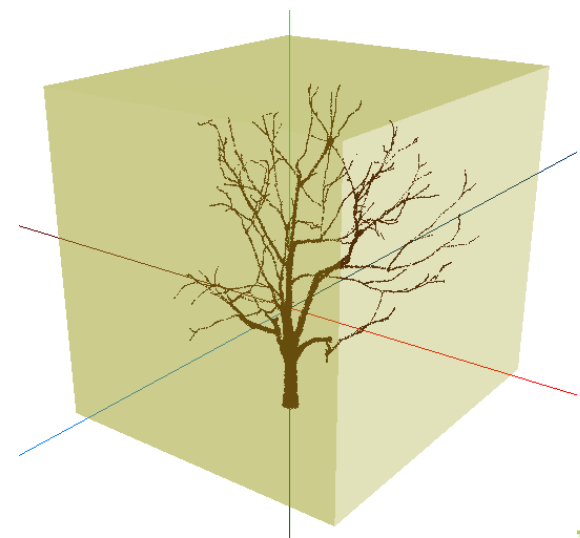
\includegraphics[width=0.3\linewidth]{box.png}}\hfill
	\subfloat[包围盒空间分块]{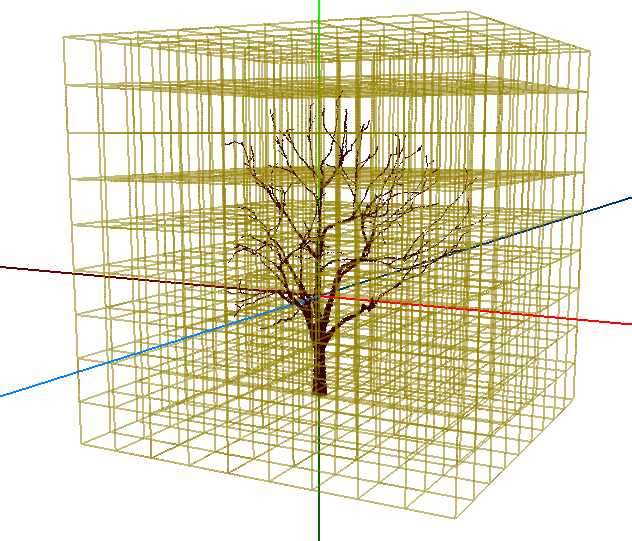
\includegraphics[width=0.3\linewidth]{voxel.png}}\hfill
	\subfloat[点云索引]{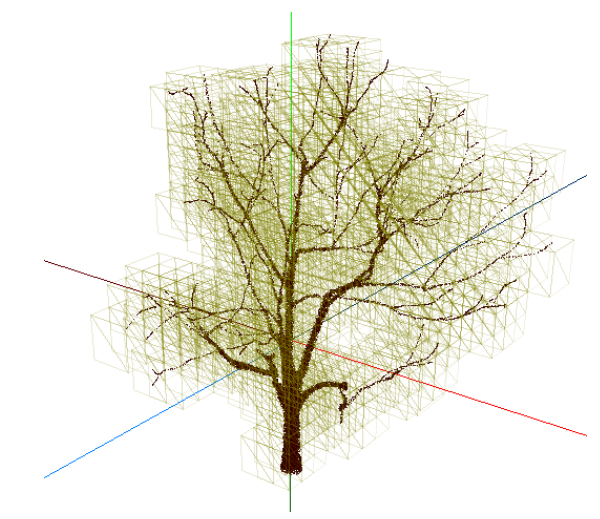
\includegraphics[width=0.3\linewidth]{index.png}}
	\caption{点云体素化}
	\label{fig:voxel}
\end{figure}

在将点云模型转化为体素模型以后,对于点云的邻域搜索便转化为了对于空间临近体素的
搜索,体素的位置就反映了点集的位置,因此不用每次搜索都遍历整个点云,而是只用将
步长范围体素中的点集遍历即可。由于体素是我们处理的基本单位,所以体素的大小也
直接决定了体素模型的精度,因此,在确保非空体素的空间连续性和效率允许的基础上,
本文建议让体素尽可能的小,以保证模型的精度。将点云模型转换为体素模型的伪代码
在算法\ref{alg:voxel}中给出。

\begin{algorithm}[H]
	\caption{点云模型体素化}
	\label{alg:voxel}
	\begin{algorithmic}[1] 
	\Require 点云模型$M$
	\Require 体素维度$d$
	\Ensure 三维体素数组$\mathbb{V}[1..d,1..d,1..d]$
	\State 初始化点云边界值$X_{max}=Y_{max}=Z_{max}=MIN\uline\quad FLOAT,X_{min}=Y_{min}=Z_{min}=MAX\uline\quad FLOAT$
	\ForAll{空间点$P(P_x,P_y,P_z) \in M$}
		\State $CheckBoundary(P)$
	\EndFor
\ForAll{空间点$P(P_x,P_y,P_z) \in M$}
\State $V_x = \frac{P_x-X_{min}}{X_{max}-X_{min}}\cdot d$
\State $V_y = \frac{P_y-Y_{min}}{Y_{max}-Y_{min}}\cdot d$
\State $V_z = \frac{P_z-Z_{min}}{Z_{max}-Z_{min}}\cdot d$
\State $\mathbb{V}[V_x, V_y, V_z] = \mathbb{V}[V_x, V_y, V_z] \bigcup \{P\} $
	\EndFor
\end{algorithmic}
\end{algorithm}

\section{三维体素泛洪确定邻域范围}
在确定了三维体素模型以后,便需要从根到叶,自底向上地对树的骨架结构进行生长。
生长的依据是已经得到的体素模型,将体素模型中点的分布作用于骨架的分支,便可以
张成骨架模型。

具体方法是将根节点置为当前节点,对其进行三维泛洪,首先对其相邻的26个体素进行泛洪,若
体素不为空,则将其加入邻域范围,若为空,则停止向该方向进行迭代。同时将加入邻域
范围的体素置为无效,表示其已经参与了泛洪,不再参与骨架的重建,这样不仅可以对算法
的结束有一个很好的约束条件,同时也可以减少重复处理的次数,加快算法的完成。然后进行下一次迭代,
对新加入的体素进行26方向的泛洪,并把有效的体素加入到邻域范围。接着比较两次迭代
体素增加的比例,如果低于设置的阈值,则停止迭代,当前的邻域范围即为三维泛洪得到
的当前节点的邻域范围。

图\ref{fig:3dfld}展示了三维体素泛洪确定邻域的步骤,三张图都延空间z轴正向投影到2D平面。
\ref{fig:3dfld}(a)为其初始状态,
即邻域范围为当前体素。其中橙色的区域表示邻域范围,蓝色的区域表示未探索区域,灰色区域
表示空的体素,而绿色区域表示已经在之前的枝干邻域。\ref{fig:3dfld}(b)表示体素泛洪经过
一次迭代以后的状态,因为体素泛洪只会对与当前邻域范围相邻的未探索区域(蓝色方块)进行扩展,
所以\ref{fig:3dfld}(a)只会向黄色箭头指向的体素进行扩展,从而得到\ref{fig:3dfld}(b)。在得到
新的邻域后,首先会计算所新增的点的数量与之前的数量的比值有没有低于阈值,如果低于阈值,则停止
邻域的扩张。最后将得到\ref{fig:3dfld}(c)中的邻域范围。

\begin{figure}[H]
	\centering
	\subfloat[初始状态(邻域范围为1个体素)]{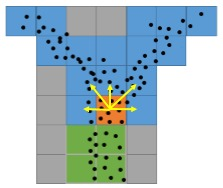
\includegraphics[height=3cm]{fld1.jpg}}\hspace{4em}
	\subfloat[第一次泛洪迭代(邻域范围为6个体素)]{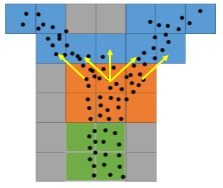
\includegraphics[height=3cm]{fld2.jpg}}\hspace{4em}
	\subfloat[第二次泛洪迭代(邻域范围为11个体素)]{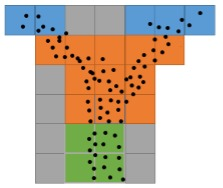
\includegraphics[height=3cm]{fld3.jpg}}
	\caption{单个体素泛洪示意图}
	\label{fig:3dfld}
\end{figure}

由于树木有多个节点,所以确定节点间的泛洪顺序十分重要。因为泛洪算法对泛洪过的区域不再进行泛洪,因此
需要将各个节点之间的相互影响降到最低。本文通过广度优先的方法,按层级对体素进行泛洪,这样就避免了子
节点的泛洪影响到叔父节点的泛洪。同时,对于同一层级的体素,将其视为多个种子点,并采取并发的泛洪,
也就是同时对它们进行泛洪,这样既提高了泛洪的效率,也使得同层级间的体素之间的影响降到最小。

图\ref{fig:flood}给出了多种子点并发泛洪确定邻域的示意图。其中蓝色方块为未泛洪体素,着红色的方块表示
已泛洪体素,橙色的小球为当前的种子点。由图可见,当前的种子点为树木的相同层级上的节点,即广度优先的
并发泛洪。

\begin{figure}[H]
	\centering
	\subfloat[步骤1]{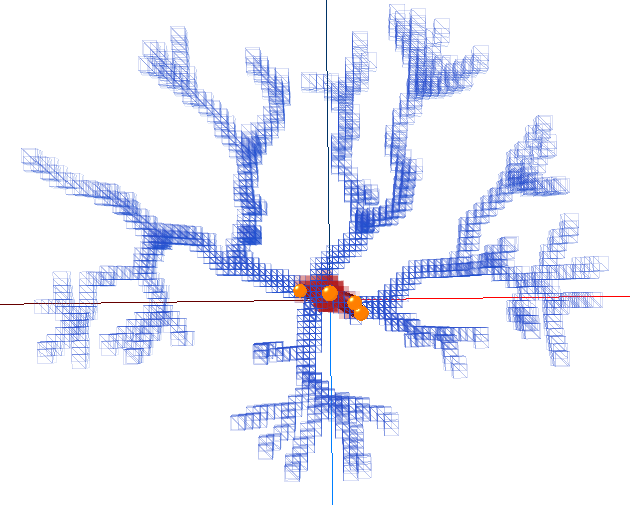
\includegraphics[width=0.4\linewidth]{seed1.png}}\hfill
	\subfloat[步骤2]{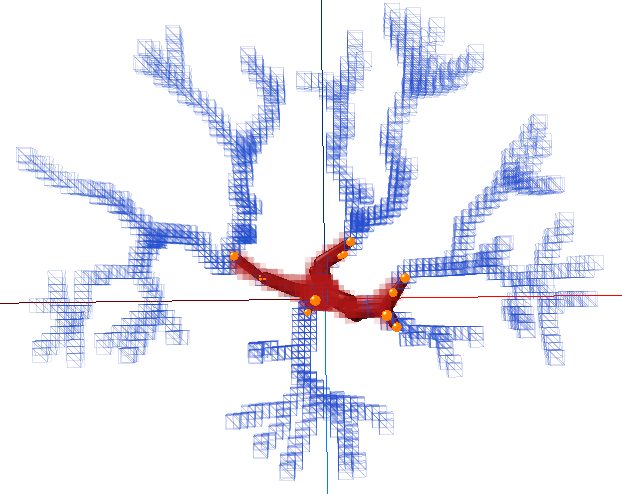
\includegraphics[width=0.4\linewidth]{seed2.png}}\hfill
	\subfloat[步骤3]{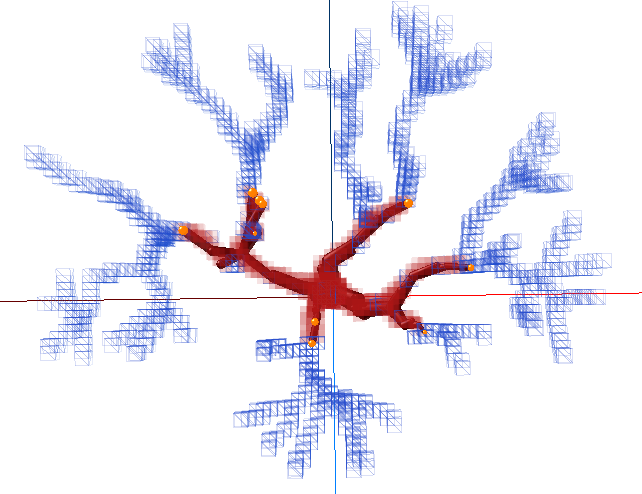
\includegraphics[width=0.4\linewidth]{seed3.png}}\hfill
	\subfloat[步骤4]{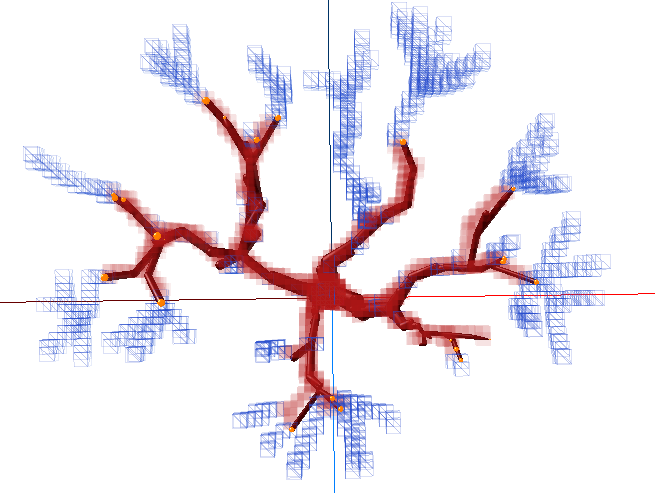
\includegraphics[width=0.4\linewidth]{seed4.png}}\hfill
	\caption{多种子点并发泛洪示意图}
	\label{fig:flood}
\end{figure}

多种子点并发体素泛洪确定邻域范围算法的伪代码在算法\ref{alg:3dfld}中给出。
\begin{algorithm}[H] 
	\caption{多种子点并发泛洪邻域探索算法}
	\label{alg:3dfld}
	\begin{algorithmic}[1]
		\Require 当前层级体素集$\mathbb{C}$,三维体素数组$\mathbb{V}[1..d,1..d,1..d]$,
		泛洪方向数组$\mathbb{D}[1..26]$,邻域范围增长比例阈值$\lambda$,最大迭代次数$num$
		\Ensure	邻域范围内体素集合$\mathbb{S}$
		\State 当前层级体素数目$n$ = $\mathbb{C}$.Count
		\State 初始化前一次泛洪体素数目数组$\mathbb{P}[1,..,n]$
		\For{i = 1 \textbf{to} $num$}
		\State 体素索引$j = 0$
		\ForAll{体素$voxel \in \mathbb{C}$}
		\State $j++$
		\State 临时体素数组$\mathbb{T}$
		\ForAll{泛洪方向$Direction \in \mathbb{D}$}
			\State $NewIndex = voxel.Index + Direction$
			\State $NewVoxel = \mathbb{V}[NewIndex.x,NewIndex.y,NewIndex.z]$
			\If{$NewVoxel$非空$\bigcap NewVoxel$有效}
				\State $\mathbb{T}.AddVoxel(NewVoxel)$
			\EndIf
		\EndFor
		\State 体素增长比例$\mu=\frac{\mathbb{T}.Count}{\mathbb{P}[j]}$
		\If{$\mu > \lambda$}
			\ForAll{$voxel \in \mathbb{T}$}
				\State S.AddVoxel(voxel)
			\EndFor
		\EndIf
		\EndFor
		\EndFor
		\State \Return $\mathbb{S}$
	\end{algorithmic}
\end{algorithm}

\section{最小二乘法线性拟合确定分支方向}
\label{subsec:leastsquares}
当得到邻域范围以后,便得到了邻域内体素在基于当前节点26个方向上的密度分布,而
每个体素内又包含着若干的点,因此等于是得到了在当前节点邻域内的点云分布情况。
接下来的工作就是怎样从各个方向的点云的分布情况抽取出核心的骨架。本文应用线性
拟合的方法来从密集的点中抽取出一条直线,作为该部分的骨架方向。

该方法首先要剔除掉那些点云密度很小的方向,以免每个节点都朝各个方向长出一些
细碎的枝条。因为这些细碎的枝条就算在此步中不剔除,到后续的轻量化的时候也不容许
它们的存在。

然后对于剩下的若干方向$d_1,d_2...d_k$,每个方向都对应着树木的一个骨架。在处理
某个方向$d_i$时,将其包含的体素中的所有点抽取出来,得到一个密集的点集$S_i$。
然后采用待定方程的办法,设直线方程为:
\begin{equation}
	\mathbf{x} = \mathbf{x_0} + \mathbf{d}t,\quad(t \in [0,\infty))
\end{equation}

其中$\mathbf{x_0}$是当前节点的坐标,$\mathbf{d}$是待拟合的直线方向。我们假设
点集$S_i$中的点$P_1,P_2,...P_m$都在直线上,则可以得到以下方程组:\\

\begin{equation} \label{eq:line}
	\left\{ 
		\begin{array}{lll}
			a_{11}d_x+a_{12}d_y+a_{13}d_z & = & b1\\
			a_{21}d_x+a_{22}d_y+a_{23}d_z & = & b2\\
			... & & \\
			a_{n1}d_x+a_{n2}d_y+a_{n3}d_z & = & bn
		\end{array}
	\right.
\end{equation}

其中具体数值未给出,注意这里的$n=3m$,因为每个点$P$可以提供三个方向的方程式。
在这个方程组中,令\\
\begin{displaymath}
	\mathbf{U}=
\left(
\begin{array}{ccc}
	a_{11} & a_{12} & a_{13}\\
	a_{21} & a_{22} & a_{23}\\
	... & ... & ...\\
	a_{n1} & a_{n2} & a_{n3}\\
\end{array}
\right)
,\quad
\mathbf{d}=
\left(
\begin{array}{c}
	d_x\\
	d_y\\
	d_z
\end{array}
\right)
,\quad
\mathbf{b}=
\left(
\begin{array}{c}
	b_1\\
	b_2\\
	...\\
	b_n
\end{array}
\right)
\end{displaymath}


在实践中,由于筛选方向上的点数较多且发散分布,由线性代数的理论知,$\mathbf{U}$是过约束的,
即$n>r$,其中$r$是矩阵$\mathbf{U}$的秩。这种情况下没有标准的解,只能找到使误差最小的向量$\mathbf{d}$,
误差定义为:\\
\begin{equation}
	E\xlongequal{def} \sum_{i=1}^n(\mathbf{d}t_i - \mathbf{x_i} + \mathbf{x_0})^2=|\mathbf{Ud}-\mathbf{b}|^2
\end{equation}

由于$E$正比于方程的均方误差,因此只要E达到最小值,那么点集相对于该直线的波动就最
小。换句话说,也就是该直线最好的模拟了该点集所表示的骨架。由线性代数的方法很容易
可以解得$\mathbf{d}=\mathbf{[(U^TU)^{-1}U^T]b}$。图\ref{fig:fitting}展示了由当前
节点(蓝色节点)分别向两个点云集合拟合出的两条直线(红色线段),这两条直线将被作为两个
分支的方向。从图中可以看出线性拟合的方法可以很好的估计出树木分枝的方向,从而准确的
恢复出树木的父子结构。

\begin{figure}[H]
	\centering
	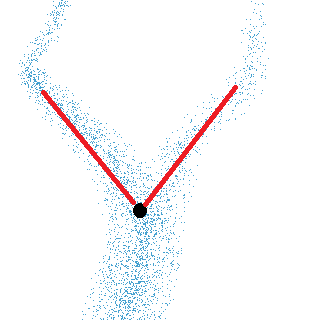
\includegraphics[height=5cm]{branch.png}
	\caption{线性拟合计算分支方向}
	\label{fig:fitting}
\end{figure}

算法\ref{alg:sklextract}给出了得到邻域信息后进行骨架方向抽取的伪代码,其中\textit{Least Squares Processing}表示运用最小二乘法进行
线性拟合。

\begin{algorithm}[H]
	\caption{基于邻域的骨架方向计算}
	\label{alg:sklextract}
	\begin{algorithmic}[1] 
		\Require 当前节点体素$V$
		\Require 骨架方向数组$\mathbb{D}[1..n]$
		\Ensure 当前节点子节点集合$\mathbb{S}$
		\ForAll{骨架方向$d\in D$}
			\State $NewChild\gets Least Squares Processing$
			\State $\mathbb{S}.AddChild(NewChild)$
		\EndFor
		\State \Return $\mathbb{S}$
	\end{algorithmic}
\end{algorithm}

\section{拟合子枝长度和半径}
树木骨架的长度和半径对树木模型的真实感有着十分显著的贡献,所以尽可能准确的获得子枝的长度和
半径信息能够有助于重建出极具真实感的树木模型。对于树木枝干半径的获取方法有许多,
主要分为根据规则生成半径和从树木点云结构中获取半径两种方式。

对于基于规则来生成半径,最简单的方法是对树木半径进行线性地递减,即$r=cR$,其中
$r$为子枝半径,$R$是父枝半径,$c$为一个线性倍数,这个倍数可以固定,也可以进行
随机的扰动从而增进多样性。Leonardo da Vinci在经过大量观察后总结出了一种更符合自然规律
的树木父子枝直径的关系公式:$D^2=\sum_{i=1}^n{d_i^2}$,其中$D$为父枝直径,$d_i$为第
$i$个子枝的直径,$n$为子枝的数量。这个公式被广泛地用于树木枝干的半径模拟。

区别于基于规则的半径生成方法,本文为了进一步提升真实感,选择在进行子枝方向抽取的同时,
同样进行半径抽取的方法。注意,用该方法的前提是点云分布须均匀化,然而基于图像进行三维重建
得到的树木点云会呈现表皮化的现象,这是由于图片上的点都是树木的表皮点,所以在得到
三维点云后,是需要进行一些修复工作的,本文用随机点填充的方法对该点云模型进行了实心化
的修复。当点云分布满足均匀化时,在对某个骨架进行拟合之后,对于拟合出来的直线,根据点
到直线的距离,可以同样根据最小二乘法拟合出骨架的半径。
该算法的伪代码在算法\ref{alg:radius}中给出。\\

\begin{algorithm}[H]
	\caption{半径拟合算法}
	\label{alg:radius}
	\begin{algorithmic}[1] 
		\Require 拟合出的当前子枝所在直线$L$
		\Require 当前子枝的点集$\mathbb{S}$
		\Ensure 当前子枝半径$R$
		\State 初始化点到直线距离数组$\mathbb{D}[1,..,n]$
		\For{$i$ = 1 \textbf{to} $n$}
		\State 点到直线距离$\mathbb{D}[i]=CalculateDistance(P, L)$
		\EndFor
		\State 拟合出使得下面式子达到最小值的半径$R$:\[ \sum_{i=1}^n (2\times \mathbb{D}[i] - R)^2  \]
		\State \Return $R$
	\end{algorithmic}
\end{algorithm}

图\ref{fig:radius}给出了三种半径求解方法的效果对比。\ref{fig:radius}(a)给出了线性衰减方法
的结果,该方法中子枝半径以父枝半径的线性倍衰减。\ref{fig:radius}(b)给出了前文提到的Leonardo
 da Vinci规则所生成的半径情况。\ref{fig:radius}(c)则采用本文中基于线性拟合的方法。
 从三者的效果中可以看出,线性衰减容易出现部分枝条生长不自然的现象,究其
 原因,还是因为一个单一的绝对的线性系数无法适用于所有的枝条,它对于某些枝条会偏大,对于另外一些
 枝条会偏小。 Leonardo规则虽然给出的是一种父子枝之间的相对关系,从一定程度上解决了线性系数单一
 绝对而导致的问题,但是它生成的树木枝干会出现过于均与化,而没有捕捉到现实中树木各个局部的特征。
 本文的方法则由于其基于对所有点的实际恢复坐标进行统计,而更加注重树木的实际局部特征情况,
 其效果也是三者之中最好的。
 \begin{figure}[H]
	\centering
	\subfloat[样本图像]{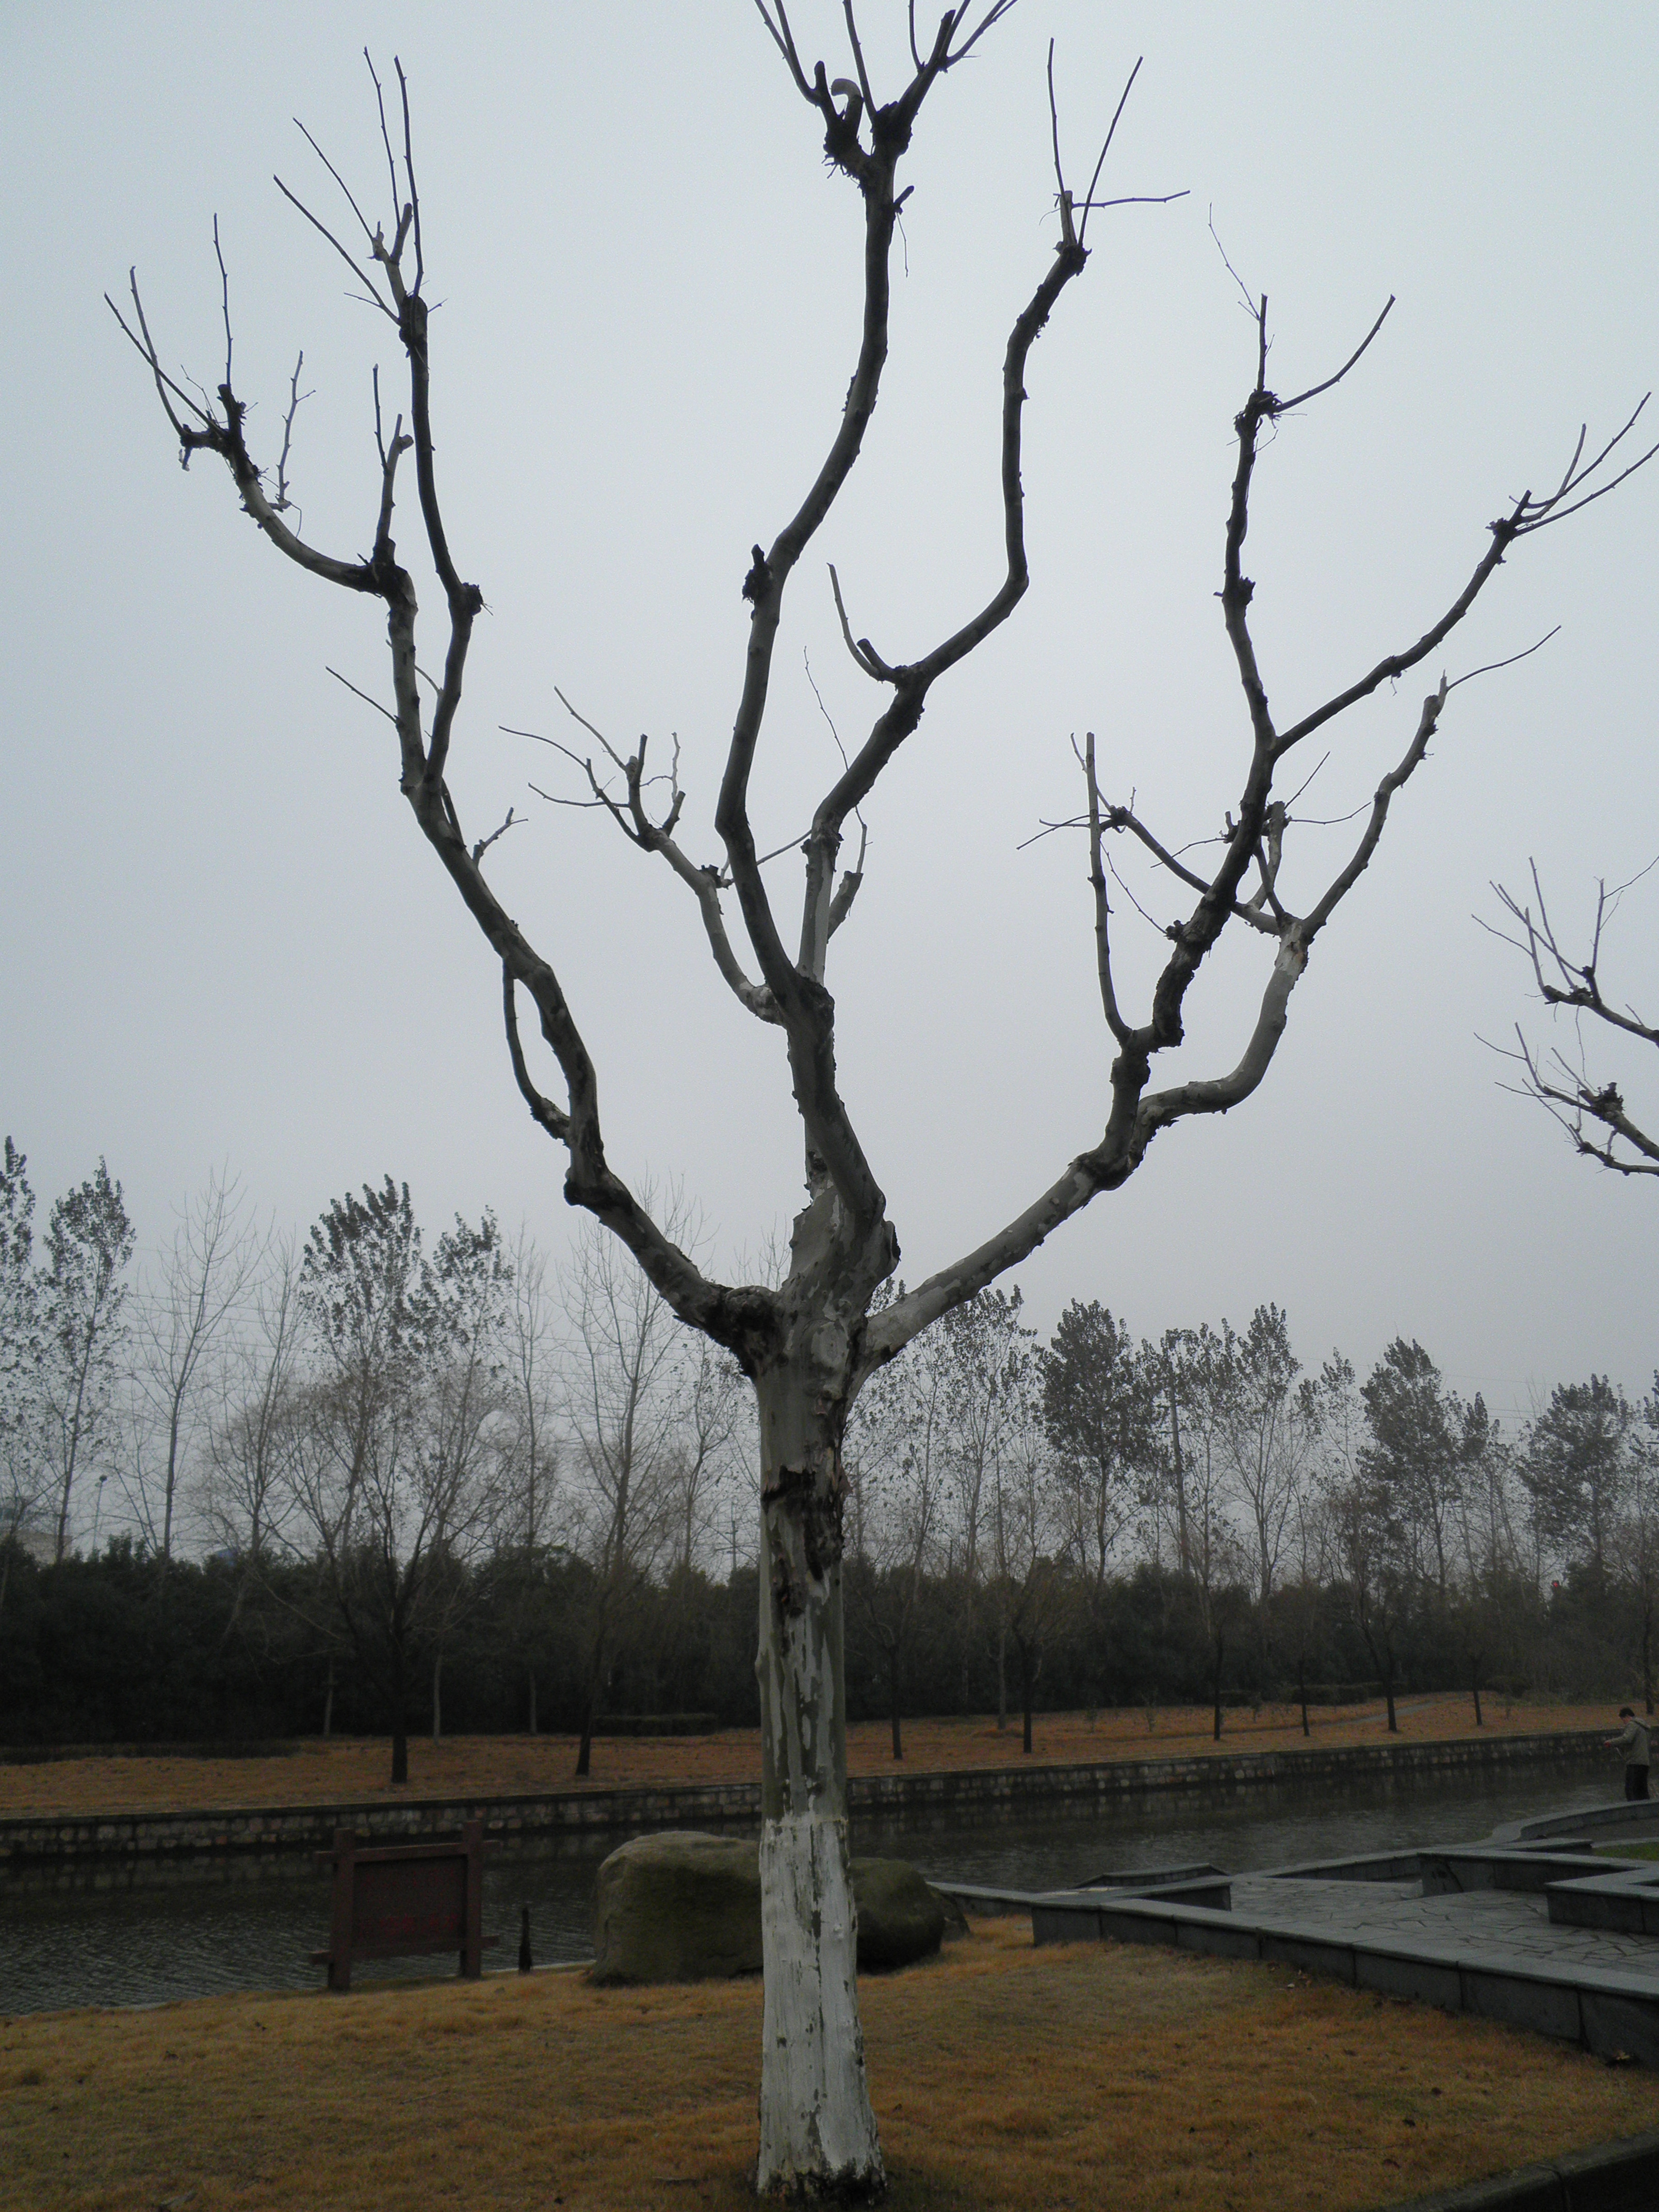
\includegraphics[height=6cm]{rsample.jpg}}\hspace{4em}
	\subfloat[线性衰减(线性衰减系数为0.6)]{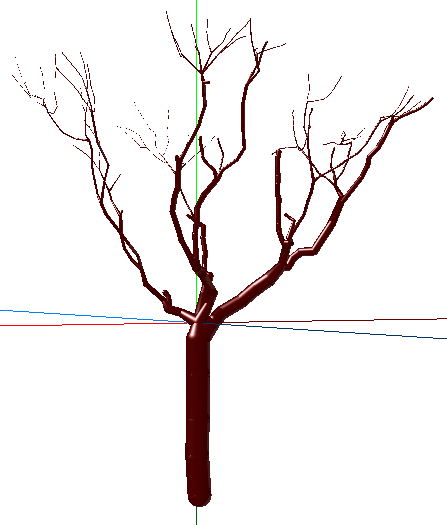
\includegraphics[height=6cm]{rlinear.png}}\hspace{4em}
	\subfloat[Leonardo规则生成($D^2=\sum_{i=1}^n{d_i^2}$)]{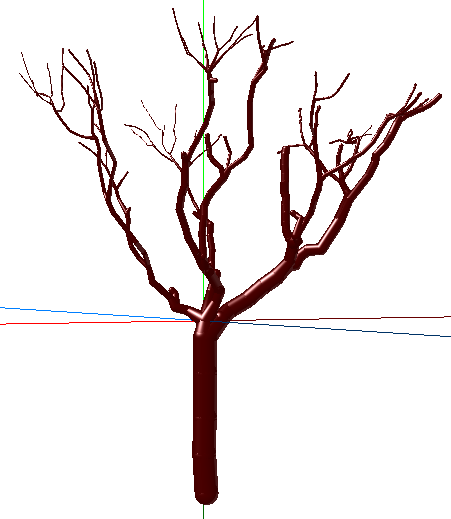
\includegraphics[height=6cm]{rsquare.png}}\hspace{4em}
	\subfloat[基于拟合的半径抽取]{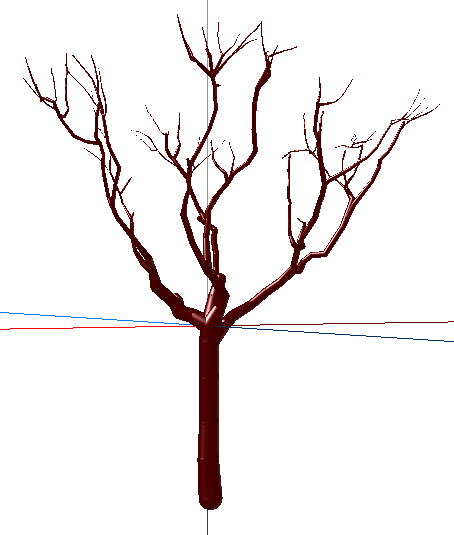
\includegraphics[height=6cm]{raffine.png}}\hspace{4em}
	\caption{三种计算半径方法效果对比}
	\label{fig:radius}
\end{figure}

对于骨架长度的估计,基于规则的生成则并不那么具有实践性,因为树木枝干的长度往往并不像半径那样
随着父子关系而递减。相反地,它地规则往往要复杂许多,而且并没有统一的规则。基于此考虑,本文并
没有对基于规则的长度估计进行实践,而是直接用与半径类似的方法,根据已拟合出的直线,试图从统计
的角度对其枝条长度做出合理的估计。一个直观而可行的方法,是将当前节点与所有该方向邻域的点的连线向量
投影到拟合出的直线方向向量上,然后根据拟合的方法得到高精确度的长度信息。
子枝长度拟合的伪代码,列在了算法\ref{alg:length}中。

\begin{algorithm}[H]
	\caption{子枝长度拟合算法}
	\label{alg:length}
	\begin{algorithmic}[1] 
		\Require 拟合出的当前子枝方向向量$L$,父节点$N$
		\Require 当前子枝的点集$\mathbb{S}$
		\Ensure 当前子枝长度$l$
		\State 初始化父节点到邻域点的向量投影长度数组$\mathbb{D}[1,..,n]$
		\For{$i$ = 1 \textbf{to} $n$}
		\State 父节点到$\mathbb{S}[i]$的向量$Dir=\mathbb{S}[i]$.Position-$N$.Position
		\State $Dir$在$L$上的投影距离$\mathbb{D}[i]$ = CalculateProjectionLength$(Dir, L)$
		\EndFor
		\State 拟合出使得下面式子达到最小值的长度$l$:\[ \sum_{i=1}^n (2\times \mathbb{D}[i] - l)^2  \]
		\State \Return $l$
	\end{algorithmic}
\end{algorithm}

\section{本章小节}

本章首先将三维重建得到的点云数据进行体素化,通过对体素求解包围盒、空间分块、点云索引的方法,将离散的点云数据
转化为连续的体素数据。

接着本章提出了基于新的树木骨架抽取方法,主要包含:\\
\begin{itemize}
	\item \textbf{多种子点的并发三维体素泛洪}: 该方法通过广度优先的方法,对树木节点进行遍历。同时对于同一层级
		上的节点,将它们作为种子点,并并发的进行三维体素的泛洪,以将节点间的相互影响降至最低。
	\item \textbf{最小二乘法拟合骨架信息}: 该方法通过最小二乘的方法,对空间的局部点云进行方向、半径和长度的
		拟合,从而以统计的方法从大量的空间点数据中抽取出有用的骨架信息。
\end{itemize}

通过本章的方法抽取出的骨架具有很高的准确性和真实感,因为它是通过统计的方法在实际的点云中进行信息的获取,相比
起其他的基于规则的信息抽取方法,该方法有明显的优势。

%

\chapter{基于枝干合并的轻量化处理}
\label{sec:branchcombine}
用基于多方向迭代与步长探索得到的三维树木骨架通常是很细致和准确的,尽管它相对于
用3DSMAX等建模工具手工建模得到的面片模型已经大大的轻量化了。但是如果应用是用于
大规模的树木建模,那么我们有必要根据应用需求进一步进行轻量化处理。

\section{L-System的尝试}
\label{subsec:lsystem}

\subsection{L-System简介}
L-System是一种并行的重写系统和正规语法,
它的结构可以用可以定义为一个3元组:\\
\[\mathbf{M} = (V, \omega, P)\]
其中:\\
\begin{itemize}
	\item $\mathbf{V}$(字母表) 表示可以被替代的字符的集合。
	\item $\mathbf{\omega}$(初始串) 表示L-System的初始状态。
	\item $\mathbf{P}$(规则集合) 表示一系列的衍生规则。
\end{itemize}
L-System可以根据这三个组成部分的不同而递归地产生形态各异的字符串。
由于L-System具有递归生长的特性,因此我们可以用L-System规则来表达一个具有自相似形态
或者分形结构的物体,比如本文所研究的对象\raisebox{0.5mm}{------}树木。

\subsection{树木模型的参数化L-System规则抽取}
球面海龟几何的提出,用参数化的L-System规则描述了树木的结构信息。在球面海龟几何中,
节点的空间几何信息用4个量(长度$l$、半径$r$、父子枝夹角$\theta$和水平转角$\phi$)
和4个扩展符号(+、-、\&、$\wedge$)来表示:
\begin{itemize}
	\item $+(l)$	表示以当前位置为起点,在当前方向上前进$l$单位个长度
	\item $!(r)$	表示设置当前节点半径为$r$
	\item $\&(\theta)$	表示设置父子枝夹角为$\theta$
	\item $\wedge(\phi)$	设置水平偏角为$\phi$
\end{itemize}
在球面海龟几何中,将每个骨架节点生成一条参数化的L-System规则,形如:\\
\begin{equation} \label{eq:turtle}
N(l,r) \rightarrow \&(\theta_0)\wedge(\phi_0)!(r) + (l)S_0(l*a_0,r*b_0)...\&(\theta_n)\wedge(\phi_n)!(r) + (l)S_n(l*a_n,r*b_n)
\end{equation}

其中N表示当前枝条,$S_0~S_n$表示当前枝条的n个子枝条,$a_i和b_i$分别表示第i个子枝条
与当前枝条的长度比和半径比,$\theta_i和\phi_i$分别表示第i个子枝条与当前枝条的空间
夹角和水平偏角。

\subsection{使用L-System进行树木轻量化建模遇到的问题}
在用参数化L-System进行树木轻量化建模时,在进行规则归纳时,有个难以克服的问题。考虑
将规则\ref{eq:turtle}中的$a_0$换成$a_0'$,则规则变成一个完全不同的规则。这意味着对于
两个分支规则,这两个规则中的子枝的长度,半径,转交,偏角等必须完全相等才能归纳为同
一个规则。而对于自然界中形态结构复杂的树木,每个分支规则几乎不可能完全等同于另一个
规则。

对上面的问题有一种解决方法就是将参数区间化,将属于同一区间的参数的值视为相同。比如
我们可以将父子枝间的转角分为18个区间,每个区间的大小为10度。但是经过分析就可以察觉,
这并没有从根本上解决这个问题。假设我们将这4个变量都各自划分为10个区间,那么规则总数
最多可以有10000个,而且在这种情况下,两个规律相同的几率也是非常小的。如果我们将分区
数量减少,则又有可能将本来差异比较大的规则归纳为一个规则,不符合真实感的要求。

所以,经过分析,这种用参数化L-System进行树木轻量化建模的方法并不适用于从骨架中去抽取
规则,而是适用于反向地用其描述的规则去产生一棵树,如台湾学者戴文凯就对单棵树的L-System
规则进行随机扰动而轻量化的建模出了整片森林。

\section{基于枝干合并的树木分级轻量化}
\label{subsec:branchmerge}
用L-System的方法抽取规则所产生的问题,从本质上看,是由于自然界中的树木形态太复杂和多变。
与其从一个本就不规则生长的事物中去抽取规则,还不如直接地在其逻辑结构上进行一系列的轻量
化操作。本文提出了分级化地对已抽取的树木骨架中对视觉影响不大的部分进行合并的方法,从而在尽可能
保证模型的视觉效果的基础上,进一步地减小树木模型的体积,使得其能更广泛地应用到WebVR、WebGame
等各个领域。

树枝的结构其实只由核心的一些枝干组成,其他的枝干只是对其结构进行微调。所以在要求进一步轻量化
的前提下,本文提出了分别从纵向和横向对树枝进行合并的方法,以去掉一些只是起到微调作用的枝干。
这种方法在尽可能保证真实感不过多丢失的前提下对树枝进行简化操作,以适应更广泛的Web应用领域。

\subsection{枝干纵向合并}

纵向合并表示从父到子,从根到页进行纵向递归式的合并。若当前节点与其父节点和子节点的夹角小于所设定
的阈值,那么则将该节点去掉,并将其子节点连接到其父节点。注意,若该节点的子节点数目不只一个,
那么我们不对它进行合并操作,因为将该节点的所有子节点加到该节点的父节点上去有违真实感。
图\ref{fig:vert}展示了树枝纵向合并过程。图\ref{fig:vert}(a)为输入的树枝骨架,并且当前节点
为\textbf{B},其父节点为\textbf{A},且只有唯一的子节点\textbf{C}。设合并角度阈值为$\alpha$,
假设\textbf{AB,BC}之间的夹角b小于合并阈值$\alpha$,那么将\textbf{B}剔除,并将\textbf{C}作为
\textbf{A}的子节点。同理,在图\ref{fig:vert}(b)中,若夹角c小于阈值$\alpha$,那么也将\textbf{AC}
和\textbf{CD}合并。在图\ref{fig:vert}(c)中,由于节点\textbf{D}有两个孩子,所以不对其进行合并
操作。

纵向合并算法的伪代码在算法\ref{alg:vertical}中给出。

\begin{figure}[H]
	\centering
	\subfloat[输入树枝骨架]{
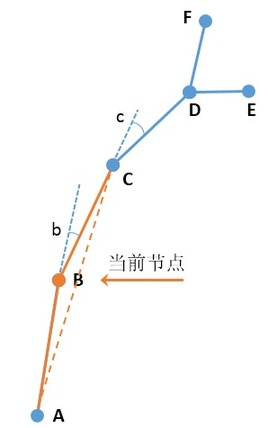
\includegraphics[height=5cm]{vert1.jpg}}
\hspace{4em}
	\subfloat[合并AB、BC]{
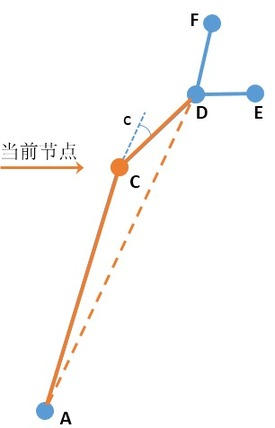
\includegraphics[height=5cm]{vert2.jpg}}
\hspace{4em}
	\subfloat[合并AC、CD]{
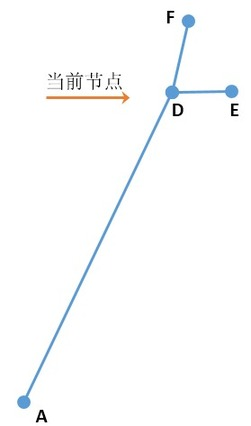
\includegraphics[height=5cm]{vert3.jpg}}
	\caption{树枝简化过程}
	\label{fig:vert}
\end{figure}

\begin{algorithm}[H]
	\caption{纵向合并枝干}
	\label{alg:vertical}
	\begin{algorithmic}[1] 
		%\Comment {根据纵向合并角度参数,以当前节点为发起点递归式地纵向合并枝干}
		\Require 纵向合并角度$\alpha$
		\Require 当前节点$N$
		\Ensure None
		\ForAll{节点$N'\in N.Children$}
		\While{$N'.ChildCount = 1$}
		\State $\vec{u} \gets N'.Position-N.Position$
		\State $\vec{v} \gets N''.Position-N'.Position$
		\State $\gamma \gets \cos^{-1}({\frac{\vec{u} \cdot \vec{v}}{|\vec{u}|\cdot|\vec{v}|}})$
		\If{$\gamma<\alpha$}
		\State $N.child \gets N.AddChild(N'')$
		\State $N.child \gets N.DeleteChild(N') $
		\EndIf
		\State $N' \gets N'.FirstChild$
		\EndWhile
		\EndFor
		\If{$N.ChildCount > 1$}
		\ForAll{节点$N'\in N.Children$}
		\State 以$N'$为当前节点递归调用该函数
		\EndFor
		\EndIf
	\end{algorithmic}
\end{algorithm}

\subsection{枝干横向合并}

横向合并指的是对非常靠近的叶子节点进行合并。之所以只对叶子节点进行合并,是
因为非叶子节点下面都有若干棵子树,若对它们进行合并,必须对它们下面的子树也进行合并。而合并子树
显然就使得真实感下降很大,因为这不只是局部微调,而是若干子树的变动。对于横向合并,不再是使用角度
来衡量两个子枝的靠近程度,而是使用子节点间的欧式距离来表示,因为合并两个角度相差小但是长度相差大的
子枝也会导致真实感的大幅下降。横向合并的伪代码在算法\ref{alg:hori}中
给出。

\begin{algorithm}[H]
	\caption{横向合并枝干}
	\label{alg:hori}
	\begin{algorithmic}[1] 
	\Require 初始化横向合并距离阈值$\mu$
	\Require 设定当前节点$N$
	\Ensure None
	\ForAll{节点对$P\in N.Children$}
		\State $N_1 \gets P.FirstNode$
		\State $N_2 \gets P.SecondNode$
		\If{$N_1.ChildCount = 0 \wedge N_2.ChildCount = 0$}
		\State $\mathbf{\vec{u}} \gets N_1.Position$
		\State $\mathbf{\vec{v}} \gets N_2.Position$
		\State $\gamma \gets |\mathbf{\vec{u}} - \mathbf{\vec{u}}|$
			\If{$\gamma<\mu$}
				\State $New\ Node\ N'$
				\State $N'.Position \gets (N_1.Position+N_2.Position)/2$
				\State $N'.Radius \gets max(N_1.Radius,N_2.Radius)$
				\State $N.child \gets N.DeleteChild(N_1)$
				\State $N.child \gets N.DeleteChild(N_2)$
				\State $N.child \gets N.AddChild(N')$
				\State 退出循环并以当前节点N重新调用该函数
			\EndIf
		\EndIf
	\EndFor
	\ForAll{节点$P\in N.Children$}
		\State 以P为当前节点递归调用该函数
	\EndFor
\end{algorithmic}
\end{algorithm}

\subsection{联合使用横纵向合并}

纵向合并和横向合并单独使用时都具有很大的局限性,因为纵向合并只能对具有单个孩子并且没有
兄弟的节点进行纵向递归地调用,而横向合并又只能对叶子节点进行兄弟级别的合并。但是将两种
合并方法联合使用,将可以从整体上对树木进行微调操作,图\ref{fig:combine}对这一想法进行了
演示。\ref{fig:combine}(a)中经过纵向的\textbf{AC,CD}合并得到\ref{fig:combine}(b)。
\ref{fig:combine}(b)中由于\textbf{D}有两个子节点,无法进行纵向合并,所以考虑进行横向
合并\textbf{DE,DF},并得到\ref{fig:combine}(c)。最后进行一次纵向合并得到\ref{fig:combine}(d)。

\begin{figure}[H]
	\centering
	\subfloat[输入枝干骨架]{
	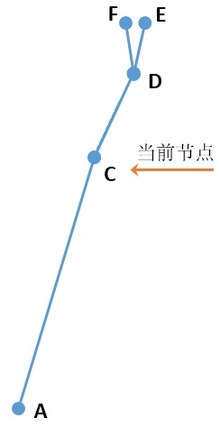
\includegraphics[height=6cm]{comb1.jpg}}
	\hspace{6em}
	\subfloat[纵向合并AC,CD]{
	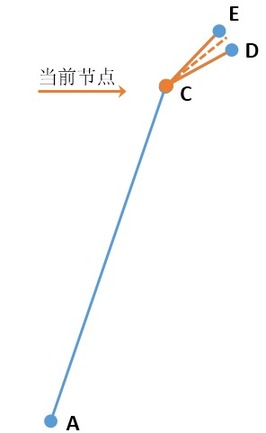
\includegraphics[height=6cm]{comb2.jpg}}
	\hspace{6em}
	\subfloat[横向合并DE,DF]{
	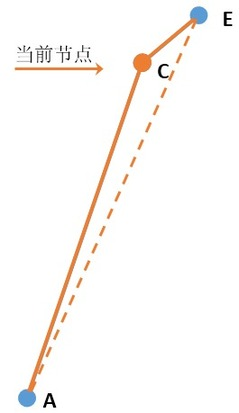
\includegraphics[height=6cm]{comb3.jpg}}
	\hspace{6em}
	\subfloat[纵向合并AD,DE]{
	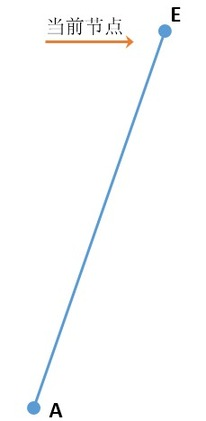
\includegraphics[height=6cm]{comb4.jpg}}
	\caption{联合使用纵向和横向合并}
	\label{fig:combine}
\end{figure}

\section{本章小节}
在得到骨架结构后,为了迎合轻量化的应用,本文对其进行轻量化操作。本章首先对传统的轻量化方法L-System进行了尝试,运用参数化
的L-System规则进行规则抽取,但是由于现实中树木的复杂性与不规则性,抽取出来的规则太多,以至于违背了轻量化的原则。于是本文
提出了基于枝干合并的轻量化方法,分别从纵向和横向对树木枝干进行合并,并对这两种方法进行有机的组合使用,以达到轻量化的目标。


%%% 其它部分
\backmatter

\makeatother

% 致谢
\cleardoublepage

%%% Local Variables:
%%% mode: latex
%%% TeX-master: "../main"
%%% End:

\begin{ack}
  衷心感谢导师 xxx 教授和物理系 xxx 副教授对本人的精心指导。他们的言传身教将使
  我终生受益。

  在美国麻省理工学院化学系进行九个月的合作研究期间,承蒙 xxx 教授热心指导与帮助,不
  胜感激。感谢 xx 实验室主任 xx 教授,以及实验室全体老师和同学们的热情帮助和支
  持!本课题承蒙国家自然科学基金资助,特此致谢。

  感谢 \tongjithesis{},它的存在让我的论文写作轻松自在了许多,让我的论文格式规整漂亮了
  许多。

\end{ack}


% 参考文献
\cleardoublepage
\bibliographystyle{tongjibib}
\bibliography{ref/refs}


% 附录
%\cleardoublepage
%\begin{appendix}
%%%% Local Variables:
%%% mode: latex
%%% TeX-master: "../main"
%%% End:

\chapter{外文资料原文}
\label{cha:engorg}
As one of the most widely used techniques in operations research, {\em
  mathematical programming} is defined as a means of maximizing a quantity known
as {\em objective function}, subject to a set of constraints represented by
equations and inequalities. Some known subtopics of mathematical programming are
linear programming, nonlinear programming, multiobjective programming, goal
programming, dynamic programming, and multilevel programming$^{[1]}$.

It is impossible to cover in a single chapter every concept of mathematical
programming. This chapter introduces only the basic concepts and techniques of
mathematical programming such that readers gain an understanding of them
throughout the book$^{[2,3]}$.


\section{Single-Objective Programming}
The general form of single-objective programming (SOP) is written
as follows,
\begin{equation}\tag*{(123)} % 如果附录中的公式不想让它出现在公式索引中,那就请
                             % 用 \tag*{xxxx}
\left\{\begin{array}{l}
\max \,\,f(x)\\[0.1 cm]
\mbox{subject to:} \\ [0.1 cm]
\qquad g_j(x)\le 0,\quad j=1,2,\cdots,p
\end{array}\right.
\end{equation}
which maximizes a real-valued function $f$ of
$x=(x_1,x_2,\cdots,x_n)$ subject to a set of constraints.

One of the outstanding contributions to mathematical programming was known as
the Kuhn-Tucker conditions\ref{eq:ktc}. In order to introduce them, let us give
some definitions. An inequality constraint $g_j(x)\le 0$ is said to be active at
a point $x^*$ if $g_j(x^*)=0$. A point $x^*$ satisfying $g_j(x^*)\le 0$ is said
to be regular if the gradient vectors $\nabla g_j(x)$ of all active constraints
are linearly independent.

%\newtheorem{mpdef}{Definition}[chapter]
%\begin{mpdef}
%In SOP, we call $x$ a decision vector, and
%$x_1,x_2,\cdots,x_n$ decision variables. The function
%$f$ is called the objective function. The set
%\begin{equation}\tag*{(456)} % 这里同理,其它不再一一指定。
%S=\left\{x\in\Re^n\bigm|g_j(x)\le 0,\,j=1,2,\cdots,p\right\}
%\end{equation}
%is called the feasible set. An element $x$ in $S$ is called a
%feasible solution.
%\end{mpdef}
%
%\newtheorem{mpdefop}[mpdef]{Definition}
%\begin{mpdefop}
%A feasible solution $x^*$ is called the optimal
%solution of SOP if and only if
%\begin{equation}
%f(x^*)\ge f(x)
%\end{equation}
%for any feasible solution $x$.
%\end{mpdefop}

Let $x^*$ be a regular point of the constraints of SOP and assume that all the
functions $f(x)$ and $g_j(x),j=1,2,\cdots,p$ are differentiable. If $x^*$ is a
local optimal solution, then there exist Lagrange multipliers
$\lambda_j,j=1,2,\cdots,p$ such that the following Kuhn-Tucker conditions hold,
\begin{equation}
\label{eq:ktc}
\left\{\begin{array}{l}
    \nabla f(x^*)-\sum\limits_{j=1}^p\lambda_j\nabla g_j(x^*)=0\\[0.3cm]
    \lambda_jg_j(x^*)=0,\quad j=1,2,\cdots,p\\[0.2cm]
    \lambda_j\ge 0,\quad j=1,2,\cdots,p.
\end{array}\right.
\end{equation}
If all the functions $f(x)$ and $g_j(x),j=1,2,\cdots,p$ are convex and
differentiable, and the point $x^*$ satisfies the Kuhn-Tucker conditions
(\ref{eq:ktc}), then it has been proved that the point $x^*$ is a global optimal
solution of SOP.

\subsection{Linear Programming}
\label{sec:lp}

If the functions $f(x),g_j(x),j=1,2,\cdots,p$ are all linear, then SOP is called
a {\em linear programming}.

The feasible set of linear is always convex. A point $x$ is called an extreme
point of convex set $S$ if $x\in S$ and $x$ cannot be expressed as a convex
combination of two points in $S$. It has been shown that the optimal solution to
linear programming corresponds to an extreme point of its feasible set provided
that the feasible set $S$ is bounded. This fact is the basis of the {\em simplex
  algorithm} which was developed by Dantzig as a very efficient method for
solving linear programming.
\begin{table}[ht]
\centering
  \centering
  \caption*{Table~1\hskip1em This is an example for manually numbered table, which
    would not appear in the list of tables}
  \label{tab:badtabular2}
  \begin{tabular}[c]{|c|m{0.8in}|c|c|c|c|c|}\hline
    \multicolumn{2}{|c|}{Network Topology} & \# of nodes &
    \multicolumn{3}{c|}{\# of clients} & Server \\\hline
    GT-ITM & Waxman Transit-Stub & 600 &
    \multirow{2}{2em}{2\%}&
    \multirow{2}{2em}{10\%}&
    \multirow{2}{2em}{50\%}&
    \multirow{2}{1.2in}{Max. Connectivity}\\\cline{1-3}
    \multicolumn{2}{|c|}{Inet-2.1} & 6000 & & & &\\\hline
    \multirow{2}{1in}{Xue} & Rui  & Ni &\multicolumn{4}{c|}{\multirow{2}*{\tongjithesis}}\\\cline{2-3}
    & \multicolumn{2}{c|}{ABCDEF} &\multicolumn{4}{c|}{} \\\hline
\end{tabular}
\end{table}

Roughly speaking, the simplex algorithm examines only the extreme points of the
feasible set, rather than all feasible points. At first, the simplex algorithm
selects an extreme point as the initial point. The successive extreme point is
selected so as to improve the objective function value. The procedure is
repeated until no improvement in objective function value can be made. The last
extreme point is the optimal solution.

\subsection{Nonlinear Programming}

If at least one of the functions $f(x),g_j(x),j=1,2,\cdots,p$ is nonlinear, then
SOP is called a {\em nonlinear programming}.

A large number of classical optimization methods have been developed to treat
special-structural nonlinear programming based on the mathematical theory
concerned with analyzing the structure of problems.
\begin{figure}[h]
  \centering
  
\includegraphics[clip]{tongji-lib-logo.jpg}
  \caption*{Figure~1\hskip1em This is an example for manually numbered figure,
    which would not appear in the list of figures}
  \label{tab:badfigure2}
\end{figure}

Now we consider a nonlinear programming which is confronted solely with
maximizing a real-valued function with domain $\Re^n$.  Whether derivatives are
available or not, the usual strategy is first to select a point in $\Re^n$ which
is thought to be the most likely place where the maximum exists. If there is no
information available on which to base such a selection, a point is chosen at
random. From this first point an attempt is made to construct a sequence of
points, each of which yields an improved objective function value over its
predecessor. The next point to be added to the sequence is chosen by analyzing
the behavior of the function at the previous points. This construction continues
until some termination criterion is met. Methods based upon this strategy are
called {\em ascent methods}, which can be classified as {\em direct methods},
{\em gradient methods}, and {\em Hessian methods} according to the information
about the behavior of objective function $f$. Direct methods require only that
the function can be evaluated at each point. Gradient methods require the
evaluation of first derivatives of $f$. Hessian methods require the evaluation
of second derivatives. In fact, there is no superior method for all
problems. The efficiency of a method is very much dependent upon the objective
function.

\subsection{Integer Programming}

{\em Integer programming} is a special mathematical programming in which all of
the variables are assumed to be only integer values. When there are not only
integer variables but also conventional continuous variables, we call it {\em
  mixed integer programming}. If all the variables are assumed either 0 or 1,
then the problem is termed a {\em zero-one programming}. Although integer
programming can be solved by an {\em exhaustive enumeration} theoretically, it
is impractical to solve realistically sized integer programming problems. The
most successful algorithm so far found to solve integer programming is called
the {\em branch-and-bound enumeration} developed by Balas (1965) and Dakin
(1965). The other technique to integer programming is the {\em cutting plane
  method} developed by Gomory (1959).

\hfill\textit{Uncertain Programming\/}\quad(\textsl{BaoDing Liu, 2006.2})

\section*{References}
\noindent{\itshape NOTE: these references are only for demonstration, they are
  not real citations in the original text.}

\begin{enumerate}[{$[$}1{$]$}]
\item Donald E. Knuth. The \TeX book. Addison-Wesley, 1984. ISBN: 0-201-13448-9
\item Paul W. Abrahams, Karl Berry and Kathryn A. Hargreaves. \TeX\ for the
  Impatient. Addison-Wesley, 1990. ISBN: 0-201-51375-7
\item David Salomon. The advanced \TeX book.  New York : Springer, 1995. ISBN:0-387-94556-3
\end{enumerate}

\chapter{外文资料的调研阅读报告或书面翻译}
\section{单目标规划}
北冥有鱼,其名为鲲。鲲之大,不知其几千里也。化而为鸟,其名为鹏。鹏之背,不知其几
千里也。怒而飞,其翼若垂天之云。是鸟也,海运则将徙于南冥。南冥者,天池也。
\begin{equation}\tag*{(123)}
 p(y|\mathbf{x}) = \frac{p(\mathbf{x},y)}{p(\mathbf{x})}=
\frac{p(\mathbf{x}|y)p(y)}{p(\mathbf{x})}
\end{equation}

吾生也有涯,而知也无涯。以有涯随无涯,殆已!已而为知者,殆而已矣!为善无近名,为
恶无近刑,缘督以为经,可以保身,可以全生,可以养亲,可以尽年。

\subsection{线性规划}
庖丁为文惠君解牛,手之所触,肩之所倚,足之所履,膝之所倚,砉然响然,奏刀騞然,莫
不中音,合于桑林之舞,乃中经首之会。
\begin{table}[ht]
\centering
  \centering
  \caption*{表~1\hskip1em 这是手动编号但不出现在索引中的一个表格例子}
  \label{tab:badtabular3}
  \begin{tabular}[c]{|c|m{0.8in}|c|c|c|c|c|}\hline
    \multicolumn{2}{|c|}{Network Topology} & \# of nodes &
    \multicolumn{3}{c|}{\# of clients} & Server \\\hline
    GT-ITM & Waxman Transit-Stub & 600 &
    \multirow{2}{2em}{2\%}&
    \multirow{2}{2em}{10\%}&
    \multirow{2}{2em}{50\%}&
    \multirow{2}{1.2in}{Max. Connectivity}\\\cline{1-3}
    \multicolumn{2}{|c|}{Inet-2.1} & 6000 & & & &\\\hline
    \multirow{2}{1in}{Xue} & Rui  & Ni &\multicolumn{4}{c|}{\multirow{2}*{\tongjithesis}}\\\cline{2-3}
    & \multicolumn{2}{c|}{ABCDEF} &\multicolumn{4}{c|}{} \\\hline
\end{tabular}
\end{table}

文惠君曰:“嘻,善哉!技盖至此乎?”庖丁释刀对曰:“臣之所好者道也,进乎技矣。始臣之
解牛之时,所见无非全牛者;三年之后,未尝见全牛也;方今之时,臣以神遇而不以目视,
官知止而神欲行。依乎天理,批大郤,导大窾,因其固然。技经肯綮之未尝,而况大坬乎!
良庖岁更刀,割也;族庖月更刀,折也;今臣之刀十九年矣,所解数千牛矣,而刀刃若新发
于硎。彼节者有间而刀刃者无厚,以无厚入有间,恢恢乎其于游刃必有余地矣。是以十九年
而刀刃若新发于硎。虽然,每至于族,吾见其难为,怵然为戒,视为止,行为迟,动刀甚微,
謋然已解,如土委地。提刀而立,为之而四顾,为之踌躇满志,善刀而藏之。”

文惠君曰:“善哉!吾闻庖丁之言,得养生焉。”


\subsection{非线性规划}
孔子与柳下季为友,柳下季之弟名曰盗跖。盗跖从卒九千人,横行天下,侵暴诸侯。穴室枢
户,驱人牛马,取人妇女。贪得忘亲,不顾父母兄弟,不祭先祖。所过之邑,大国守城,小
国入保,万民苦之。孔子谓柳下季曰:“夫为人父者,必能诏其子;为人兄者,必能教其弟。
若父不能诏其子,兄不能教其弟,则无贵父子兄弟之亲矣。今先生,世之才士也,弟为盗
跖,为天下害,而弗能教也,丘窃为先生羞之。丘请为先生往说之。”
\begin{figure}[h]
  \centering
  
\includegraphics{hello}
  \caption*{图~1\hskip1em 这是手动编号但不出现索引中的图片的例子}
  \label{tab:badfigure3}
\end{figure}

柳下季曰:“先生言为人父者必能诏其子,为人兄者必能教其弟,若子不听父之诏,弟不受
兄之教,虽今先生之辩,将奈之何哉?且跖之为人也,心如涌泉,意如飘风,强足以距敌,
辩足以饰非。顺其心则喜,逆其心则怒,易辱人以言。先生必无往。”

孔子不听,颜回为驭,子贡为右,往见盗跖。

\subsection{整数规划}
盗跖乃方休卒徒大山之阳,脍人肝而餔之。孔子下车而前,见谒者曰:“鲁人孔丘,闻将军
高义,敬再拜谒者。”谒者入通。盗跖闻之大怒,目如明星,发上指冠,曰:“此夫鲁国之
巧伪人孔丘非邪?为我告之:尔作言造语,妄称文、武,冠枝木之冠,带死牛之胁,多辞缪
说,不耕而食,不织而衣,摇唇鼓舌,擅生是非,以迷天下之主,使天下学士不反其本,妄
作孝弟,而侥幸于封侯富贵者也。子之罪大极重,疾走归!不然,我将以子肝益昼餔之膳。”


\chapter{其它附录}
其它附录的内容可以放到这里,当然如果你愿意,可以把这部分也放到独立的文件中,然后
将其\verb|\input| 到主文件中。
\section{测试附录}

%\end{appendix}

% 个人简历
%\cleardoublepage
%\begin{resume}

  \resumeitem{个人简历}

  xxxx 年 xx 月 xx 日出生于 xx 省 xx 县。
  
  xxxx 年 9 月考入 xx 大学 xx 系 xx 专业,xxxx 年 7 月本科毕业并获得 xx 学士学位。
  
  xxxx 年 9 月免试进入 xx 大学 xx 系攻读 xx 学位至今。

  \resumeitem{发表的学术论文} % 发表的和录用的合在一起

  \begin{enumerate}[{[}1{]}]
  \item Yang Y, Ren T L, Zhang L T, et al. Miniature microphone with silicon-
    based ferroelectric thin films. Integrated Ferroelectrics, 2003,
    52:229-235. (SCI 收录, 检索号:758FZ.)
  \item 杨轶, 张宁欣, 任天令, 等. 硅基铁电微声学器件中薄膜残余应力的研究. 中国机
    械工程, 2005, 16(14):1289-1291. (EI 收录, 检索号:0534931 2907.)
  \item 杨轶, 张宁欣, 任天令, 等. 集成铁电器件中的关键工艺研究. 仪器仪表学报,
    2003, 24(S4):192-193. (EI 源刊.)
  \item Yang Y, Ren T L, Zhu Y P, et al. PMUTs for handwriting recognition. In
    press. (已被 Integrated Ferroelectrics 录用. SCI 源刊.)
  \item Wu X M, Yang Y, Cai J, et al. Measurements of ferroelectric MEMS
    microphones. Integrated Ferroelectrics, 2005, 69:417-429. (SCI 收录, 检索号
    :896KM.)
  \item 贾泽, 杨轶, 陈兢, 等. 用于压电和电容微麦克风的体硅腐蚀相关研究. 压电与声
    光, 2006, 28(1):117-119. (EI 收录, 检索号:06129773469.)
  \item 伍晓明, 杨轶, 张宁欣, 等. 基于MEMS技术的集成铁电硅微麦克风. 中国集成电路, 
    2003, 53:59-61.
  \end{enumerate}

  \resumeitem{研究成果} % 有就写,没有就删除
  \begin{enumerate}[{[}1{]}]
  \item 任天令, 杨轶, 朱一平, 等. 硅基铁电微声学传感器畴极化区域控制和电极连接的
    方法: 中国, CN1602118A. (中国专利公开号.)
  \item Ren T L, Yang Y, Zhu Y P, et al. Piezoelectric micro acoustic sensor
    based on ferroelectric materials: USA, No.11/215, 102. (美国发明专利申请号.)
  \end{enumerate}
\end{resume}


\end{document}
